%==============================================================================
\chapter{Grensvlakken en materialen}
\label{ch:grensvlakken}\label{ch:oppervlakte}\label{ch:vastestof}\label{ch:kristallografie}
%==============================================================================

\section{Waarom grensvlakken en vaste stoffen samen?}
\label{sec:grensvlakken-inleiding}

Tot nu toe beschouwden we homogene fasen: een gas, een vloeistof, een mengsel. In de procesindustrie gebeurt het belangrijkste werk echter vaak aan een \emph{grensvlak}. Een katalysator werkt enkel aan zijn oppervlak, een adsorbens houdt moleculen vast aan de wand van zijn poriën, een elektrode wisselt elektronen uit aan het contact met de elektrolyt (hoofdstuk~\ref{ch:elektrochemie}), en een emulsie of verf blijft stabiel dankzij moleculen die zich aan een grensvlak ophopen. Welk oppervlak een vaste stof aanbiedt, en hoe dat oppervlak eruitziet, wordt bepaald door haar kristalstructuur, haar defecten en haar korrelgrootte. Daarom behandelen we grensvlakken en vaste stoffen in \'e\'en hoofdstuk.

Hoe belangrijk het oppervlak wordt, hangt af van de grootte. Een bol met diameter $d$ en dichtheid $\rho$ heeft een \emph{specifiek oppervlak}
\begin{equation}
a_s = \frac{6}{\rho\,d}.
\label{eq:specifiek-oppervlak}
\end{equation}
Een glasparel van \SI{1}{\milli\metre} heeft amper \SI{0.003}{\metre\squared\per\gram}; poeder van \SI{1}{\micro\metre} al \SI{3}{\metre\squared\per\gram}. Actieve kool haalt \SI{1000}{\metre\squared\per\gram}, het oppervlak van vier tennisvelden in een theelepel, niet door kleine korrels maar door een netwerk van poriën van enkele nanometer. Bij een platinadeeltje van \SI{2}{\nano\metre} ligt ongeveer de helft van de atomen aan het oppervlak: elk atoom telt mee voor de katalyse.

\begin{toepassing}{Centrale case: een katalysatorkorrel}
In de zwavelzuurfabriek, de stoomreformer en de uitlaat van een auto (hoofdstuk~\ref{ch:reagerend}) zit de katalysator op een poreuze drager, bijvoorbeeld een korrel $\gamma$-$\mathrm{Al_2O_3}$ van enkele millimeter met poriën van ongeveer \SI{10}{\nano\metre} en een specifiek oppervlak van \SI{200}{\metre\squared\per\gram}. Daarop zitten platinadeeltjes van enkele nanometer. In dit hoofdstuk beantwoorden we de vragen die een ingenieur over zo'n korrel stelt: hoe meet je dat oppervlak (\S~\ref{sec:bet}), waarom vullen de poriën zich met vloeistof bij een druk onder de dampdruk (\S~\ref{sec:kelvin}), hoe sterk hechten de reactanten aan het oppervlak (\S~\ref{sec:langmuir-isotherm-kinetiek}), en hoe weet je welke kristalvorm en hoe grote metaaldeeltjes je hebt (\S~\ref{sec:xrd}). Een tweede, alledaagse case loopt door de delen over surfactanten en colloïden: hoe een wasmiddel vet van textiel haalt.
\end{toepassing}

\section{Oppervlaktespanning}
\label{sec:oppervlaktespanning}

De \emph{oppervlaktespanning} $\sigma$ (of $\gamma$) is de arbeid die nodig is om de oppervlakte van een vloeistof met \'e\'en eenheid te vergroten:
\begin{equation}
\boxed{\;\sigma = \left(\frac{\partial G}{\partial A}\right)_{T,p,n}\;}
\label{eq:oppervlaktespanning}
\end{equation}
De eenheid is \si{\joule\per\metre\squared} of equivalent \si{\newton\per\metre}. De oppervlaktespanning is dus de toename van de Gibbs-vrije energie per eenheid oppervlakte, een directe toepassing van de thermodynamica uit hoofdstuk~\ref{ch:spontaniteit}.

Voor water bedraagt $\sigma \approx \SI{72}{\milli\newton\per\metre}$ bij \SI{20}{\celsius}; voor ethanol $\sigma \approx \SI{22}{\milli\newton\per\metre}$; voor kwik $\sigma \approx \SI{485}{\milli\newton\per\metre}$. Hoge oppervlaktespanning wijst op sterke cohesie tussen de moleculen (hoofdstuk~\ref{ch:intermoleculair}).

\subsection{Temperatuursafhankelijkheid}

Naarmate de temperatuur stijgt, worden de intermoleculaire krachten relatief zwakker ten opzichte van de thermische beweging. De oppervlaktespanning neemt dus af met de temperatuur, en nadert nul bij het kritische punt waar het onderscheid tussen vloeistof en damp verdwijnt (hoofdstuk~\ref{ch:niet-reagerend}, \S~\ref{sec:kritisch-punt}). Een empirische correlatie is die van E\"otv\"os:
\begin{equation}
\sigma V_m^{2/3} = k\,(T_c - T),
\end{equation}
waarin $V_m$ het molaire volume, $T_c$ de kritische temperatuur en $k$ een universele constante is.

\subsection{De vergelijking van Young--Laplace}

Een gekromd grensvlak heeft een drukverschil ten gevolge van de oppervlaktespanning. Voor een bolle bel met straal $r$ geldt de \emph{vergelijking van Young--Laplace}:
\begin{equation}
\boxed{\;\Delta p = \frac{2\sigma}{r}\;}
\label{eq:young-laplace}
\end{equation}
Hoe kleiner de bel, hoe groter de binnendruk. Dit verklaart waarom kleine bellen in een vloeistof spontaan in grotere bellen samensmelten (Ostwald-rijping).

\begin{voorbeeld}{Druk in een zeepbel}
Een zeepbel met straal $r = \SI{1}{\milli\metre}$ heeft een oppervlaktespanning van $\sigma = \SI{25}{\milli\newton\per\metre}$ (verlaagd door zeep). De binnendruk bedraagt:
\[
\Delta p = \frac{2(\SI{0.025}{\newton\per\metre})}{\SI{1e-3}{\metre}} = \SI{50}{\pascal}.
\]
Voor een longblaasje met $r = \SI{50}{\micro\metre}$ in water ($\sigma = \SI{72}{\milli\newton\per\metre}$, zonder surfactant):
\[
\Delta p = \frac{2(\SI{0.072}{\newton\per\metre})}{\SI{50e-6}{\metre}} = \SI{2880}{\pascal} \approx \SI{0.029}{\bar}.
\]
Dit verklaart de fysiologische noodzaak van longsurfactant (fosfolipiden), die de oppervlaktespanning drastisch verlaagt en de ademhaling mogelijk maakt.
\end{voorbeeld}

\subsection{Capillariteit}

Wanneer een vloeistof in contact komt met een vaste wand, kan de vloeistof opstijgen (hydrofiel) of dalen (hydrofoob). De \emph{stijghoogte} in een capillair met straal $r$ wordt gegeven door de wet van Jurin:
\begin{equation}
\boxed{\;h = \frac{2\sigma \cos\theta}{\rho g r}\;}
\end{equation}
waarin $\theta$ de contacthoek, $\rho$ de dichtheid en $g$ de valversnelling zijn. Voor volledige bevochtiging ($\theta = 0$) stijgt water in een capillair van \SI{0.1}{\milli\metre} met ongeveer \SI{15}{\centi\metre}.

\subsection{Bevochtiging en de contacthoek}
\label{sec:contacthoek}

Leg een druppel op een vaste stof en hij spreidt uit of blijft als een bolletje liggen. Aan de rand van de druppel trekken drie grensvlakspanningen aan het contactpunt: vast--gas ($\sigma_{sg}$), vast--vloeistof ($\sigma_{sl}$) en vloeistof--gas ($\sigma_{lg}$). Evenwicht langs het oppervlak geeft de \emph{vergelijking van Young}:
\begin{equation}
\boxed{\;\sigma_{sg} = \sigma_{sl} + \sigma_{lg}\cos\theta\;}
\label{eq:young}
\end{equation}
met $\theta$ de \emph{contacthoek}, gemeten door de vloeistof (figuur~\ref{fig:contacthoek}). Een hoge oppervlakte-energie van de vaste stof (glas, metaal, gereinigd met een coronabehandeling) geeft een kleine contacthoek: de vloeistof bevochtigt. Een lage oppervlakte-energie (PTFE, paraffine, siliconen) geeft $\theta > 90^\circ$. Dezelfde intermoleculaire krachten die in hoofdstuk~\ref{ch:intermoleculair} (\S~\ref{sec:im-toepassingen}) bepaalden of een lijm hecht, bepalen hier of verf, inkt of een coating zich mooi spreidt.

\begin{figure}[htb]
    \centering
    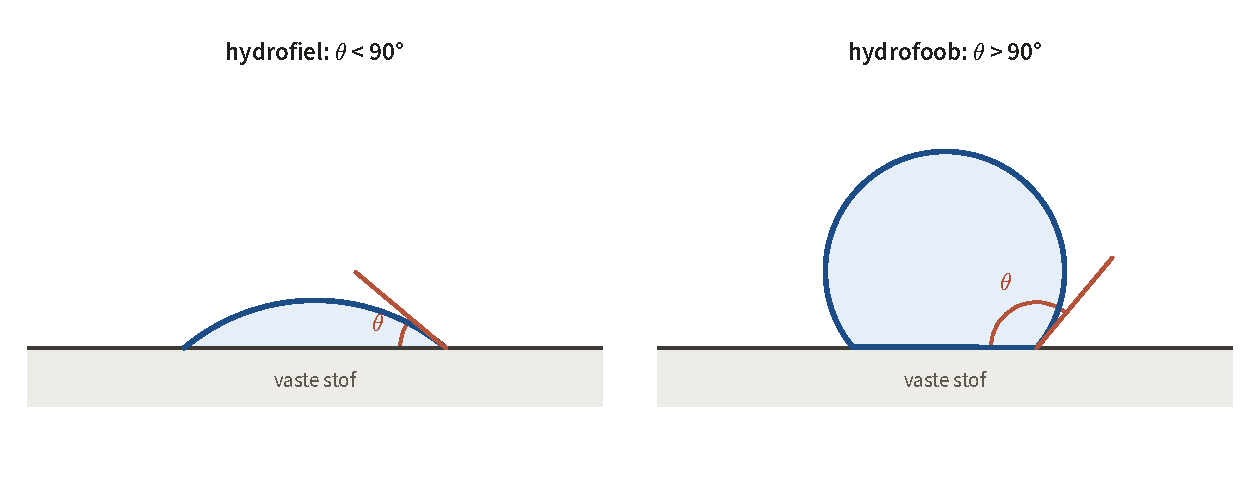
\includegraphics[width=0.85\linewidth]{Figuren/contacthoek}
    \caption{Een druppel op een hydrofiel oppervlak (links, kleine contacthoek) en op een hydrofoob oppervlak (rechts, grote contacthoek). De hoek wordt gemeten door de vloeistof, tussen het vaste oppervlak en de raaklijn aan het vloeistofoppervlak.}
    \label{fig:contacthoek}
\end{figure}

\subsection{Kleine druppels en nauwe poriën: de vergelijking van Kelvin}
\label{sec:kelvin}

Een gekromd oppervlak verandert ook de dampdruk. Een molecule in een kleine druppel staat onder de extra druk $2\sigma/r$ van Young--Laplace; zijn chemische potentiaal stijgt met $V_m\,\Delta p$ (hoofdstuk~\ref{ch:niet-reagerend}). Evenwicht met de damp vraagt dan een hogere dampdruk:
\begin{equation}
\boxed{\;\ln\frac{p}{p_\mathrm{sat}} = \pm\frac{2\sigma V_m}{rRT}\;}
\label{eq:kelvin}
\end{equation}
met het plusteken voor een bolle druppel en het minteken voor een holle meniscus in een porie die bevochtigd wordt. Dit is de \emph{vergelijking van Kelvin}.

\begin{voorbeeld}{Mist, silicagel en een vochtige katalysator}
Voor water bij \SI{20}{\celsius} is $2\sigma V_m/RT = 2(0.072)(\num{1.8e-5})/(8.314\cdot293) = \SI{1.06e-9}{\metre}$.
\begin{itemize}
\item Een druppeltje met $r = \SI{10}{\nano\metre}$: $\ln(p/p_\mathrm{sat}) = 0.106$, dus $p = 1.11\,p_\mathrm{sat}$. Zo'n druppel verdampt in lucht die net verzadigd is. Wolken vormen zich daarom pas op stofdeeltjes of zoutkristalletjes (condensatiekernen), en zuivere lucht kan sterk oververzadigd raken.
\item Een porie met $r = \SI{2}{\nano\metre}$ en volledige bevochtiging: $\ln(p/p_\mathrm{sat}) = -0.53$, dus $p = 0.59\,p_\mathrm{sat}$. Bij een relatieve vochtigheid van \SI{59}{\percent} condenseert water al in zulke poriën. Dat is het werkingsprincipe van silicagel als droogmiddel, en de reden waarom een poreuze katalysatordrager in vochtige lucht water opneemt. Omgekeerd gebruikt men deze \emph{capillaire condensatie} om de poriegrootteverdeling van een materiaal te meten.
\end{itemize}
\end{voorbeeld}

\section{Adsorptie aan grensvlakken}
\label{sec:adsorptie-grensvlakken}

\emph{Adsorptie} is de ophoping van een stof aan een grensvlak, zonder dat ze in de bulk doordringt (dat heet absorptie). Het molecule dat zich hecht, heet het \emph{adsorbaat}; de vaste stof het \emph{adsorbens}. Adsorptie is de eerste stap van elke heterogeen gekatalyseerde reactie (hoofdstuk~\ref{ch:kinetiek}) en de basis van belangrijke scheidingsprocessen: gasdroging, waterzuivering met actieve kool, en de productie van zuivere waterstof, stikstof of zuurstof.

\subsection{Fysisorptie en chemisorptie}
\label{sec:fysisorptie-chemisorptie}

Adsorptie van een molecule aan een oppervlak kan op twee fundamenteel verschillende manieren gebeuren:
\begin{itemize}
\item \textbf{Fysisorptie}: het molecule wordt via zwakke Van der Waals-krachten (hoofdstuk~\ref{ch:intermoleculair}) aan het oppervlak gebonden. De adsorptie-enthalpie is klein (typisch \SIrange{5}{40}{\kilo\joule\per\mole}, vergelijkbaar met een verdampingsenthalpie), niet-specifiek, en kan in meerdere lagen optreden (\S~\ref{sec:bet}). Fysisorptie is snel, reversibel, en neemt toe bij lagere temperatuur.
\item \textbf{Chemisorptie}: het molecule vormt een echte chemische binding (covalent of ionogen, hoofdstuk~\ref{ch:kwantum}) met het oppervlak, vaak gepaard met dissociatie (bijvoorbeeld $\mathrm{H_2}\to2\,\mathrm{H}_{\text{ads}}$). De adsorptie-enthalpie is groot (typisch \SIrange{40}{800}{\kilo\joule\per\mole}), sterk specifiek voor bepaalde oppervlakteatomen, en beperkt tot \'e\'en enkele monolaag. Chemisorptie is de stap die eigenlijk verantwoordelijk is voor katalytische activiteit: de chemische binding tussen reagens en oppervlak verzwakt de interne bindingen van het reagens (bijvoorbeeld de sterke $\mathrm{N\equiv N}$-binding bij Haber--Bosch), wat exact de activeringsenergie van de daaropvolgende reactiestap verlaagt.
\end{itemize}
Beide vormen van adsorptie zijn, net als elke andere fase-overgang (hoofdstuk~\ref{ch:niet-reagerend}), exotherm: een molecule dat zich aan een oppervlak bindt, verliest bewegingsvrijheid (negatieve adsorptie-entropie, hoofdstuk~\ref{ch:spontaniteit}), zodat enkel een negatieve adsorptie-enthalpie een spontaan ($\Delta G_{\text{ads}}<0$) proces kan opleveren.

\subsection{Het adsorptie-evenwicht en de Langmuir-isotherme}
\label{sec:langmuir-isotherm-kinetiek}

Om adsorptie en later de kinetiek van een oppervlaktereactie te beschrijven, hebben we een kwantitatieve uitdrukking nodig voor de \emph{bedekkingsgraad} $\theta$ van het oppervlak: de fractie van de beschikbare adsorptieplaatsen die bezet is, met $0\leq\theta\leq1$.

Beschouw een gas $A$ met partiële druk $p_A$ boven een oppervlak met een vast aantal adsorptieplaatsen. We veronderstellen (het model van \emph{Langmuir}):
\begin{itemize}
\item alle adsorptieplaatsen zijn energetisch equivalent;
\item elke plaats kan hoogstens \'e\'en molecule dragen (monolaagadsorptie);
\item geadsorbeerde moleculen be\"invloeden elkaar niet.
\end{itemize}
De snelheid van adsorptie is evenredig met zowel de partiële druk (botsingsfrequentie met het oppervlak) als de fractie \emph{vrije} plaatsen $(1-\theta)$:
\[
r_{\text{ads}} = k_a\,p_A\,(1-\theta).
\]
De snelheid van desorptie is evenredig met de fractie \emph{bezette} plaatsen:
\[
r_{\text{des}} = k_d\,\theta.
\]
In evenwicht zijn beide snelheden gelijk, $r_{\text{ads}}=r_{\text{des}}$:
\[
k_a\,p_A(1-\theta) = k_d\,\theta \quad\Longrightarrow\quad \theta = \frac{k_a\,p_A}{k_d+k_a\,p_A}.
\]
Met de \emph{adsorptie-evenwichtsconstante} $K_A\equiv k_a/k_d$ (met dimensie druk$^{-1}$) volgt de \emph{Langmuir-isotherme}:
\begin{equation}
\boxed{\;\theta_A = \frac{K_A\,p_A}{1+K_A\,p_A}.\;}
\label{eq:langmuir-isotherm}
\end{equation}
Bij lage druk ($K_Ap_A\ll1$) is $\theta_A\approx K_Ap_A$: de bedekking stijgt lineair met de druk. Bij hoge druk ($K_Ap_A\gg1$) is $\theta_A\to1$: het oppervlak is volledig verzadigd en verdere drukverhoging heeft nauwelijks effect --- hetzelfde verzadigingsgedrag dat in hoofdstuk~\ref{ch:kinetiek} terugkomt bij enzymen (Michaelis--Menten).

Voor twee competitief adsorberende gassen $A$ en $B$ geldt op dezelfde manier:
\begin{equation}
\theta_A = \frac{K_Ap_A}{1+K_Ap_A+K_Bp_B}, \qquad \theta_B = \frac{K_Bp_B}{1+K_Ap_A+K_Bp_B}.
\label{eq:langmuir-competitief}
\end{equation}
Een sterker adsorberende component (grotere $K$) verdringt een zwakker adsorberende component van het oppervlak Dat effect bepaalt de snelheid van oppervlaktereacties (hoofdstuk~\ref{ch:kinetiek}) en het vergiftigen van katalysatoren, bijvoorbeeld door CO op het platina van een brandstofcel.

De constante $K$ is een evenwichtsconstante en volgt dus de vergelijking van Van 't Hoff (hoofdstuk~\ref{ch:reagerend}): omdat adsorptie exotherm is, daalt $K$ bij stijgende temperatuur. Een adsorbens laadt men daarom koud en onder druk, en regenereert men warm of bij lage druk.

\begin{toepassing}{Zuivere waterstof met drukwisseladsorptie (PSA)}
Na de stoomreformer en de shiftreactoren (hoofdstuk~\ref{ch:reagerend}, \S~\ref{sec:case-waterstof}) bevat het gas ongeveer \SI{75}{\percent} H$_2$, de rest is vooral CO$_2$, met wat CH$_4$, CO en water. In een PSA-eenheid stroomt dit gas bij ongeveer \SI{25}{\bar} door kolommen met actieve kool en zeoliet. CO$_2$, CH$_4$ en CO adsorberen sterk (grote $K$), H$_2$ nauwelijks: het verlaat de kolom met een zuiverheid van \SI{99.999}{\percent}. Is een kolom vol, dan laat men de druk zakken tot net boven \SI{1}{\bar}: volgens de Langmuir-isotherme komt het grootste deel van het adsorbaat weer vrij. Enkele kolommen wisselen elkaar af in cycli van enkele minuten. Hetzelfde principe levert stikstof uit lucht (koolstofmoleculaire zeven) en zuurstof voor zuurstofconcentrators in de zorg (zeolieten die N$_2$ sterker binden dan O$_2$).
\end{toepassing}

\begin{figure}[htb]
    \centering
    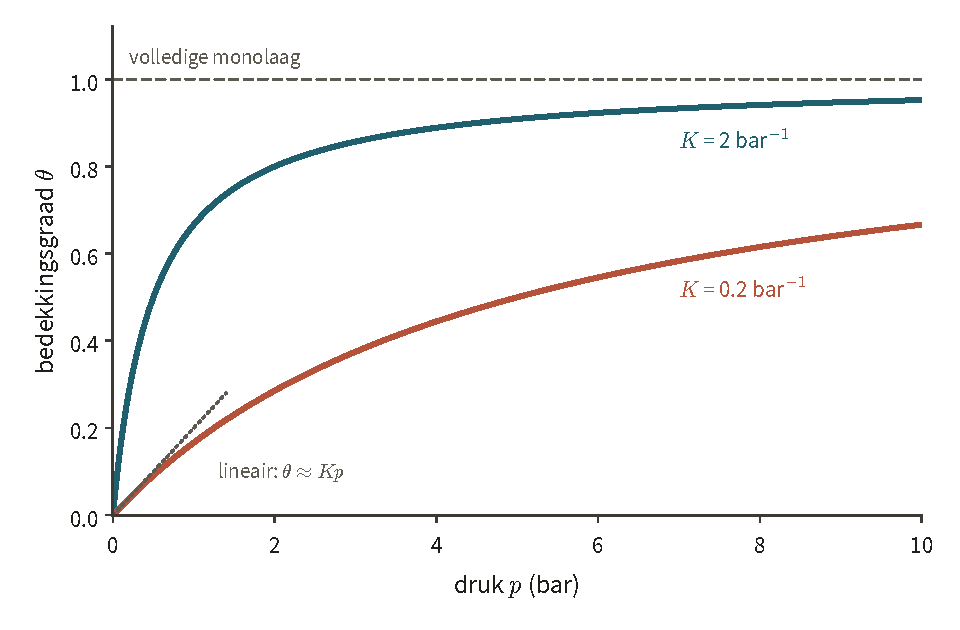
\includegraphics[width=0.7\linewidth]{Figuren/langmuir_isotherm}
    \caption{De Langmuir-isotherme (vergelijking~\eqref{eq:langmuir-isotherm}) voor twee waarden van de adsorptieconstante. Bij lage druk stijgt de bedekking lineair, bij hoge druk nadert ze een volledige monolaag. Een sterker adsorberend gas (grotere $K$) verzadigt het oppervlak al bij lage druk.}
    \label{fig:langmuir-isotherm}
\end{figure}

\subsection{De BET-isotherme: voorbij de monolaag}
\label{sec:bet}

De Langmuir-isotherme veronderstelt monolaagadsorptie --- gerechtvaardigd voor chemisorptie, maar niet voor fysisorptie, waar bij voldoende hoge relatieve druk meerdere lagen fysisorberen (vergelijkbaar met condensatie, hoofdstuk~\ref{ch:niet-reagerend}). Brunauer, Emmett en Teller (1938) breidden het Langmuir-model uit tot multilaagadsorptie, wat leidt tot de \emph{BET-isotherme}:
\begin{equation}
\frac{V}{V_m} = \frac{C\,x}{(1-x)\bigl[1-x+Cx\bigr]}, \qquad x=\frac{p}{p_{\text{sat}}},
\label{eq:bet}
\end{equation}
waarin $V$ het geadsorbeerde volume, $V_m$ het volume van precies \'e\'en monolaag, $p_{\text{sat}}$ de verzadigingsdampdruk van het adsorberende gas bij de gegeven temperatuur (hoofdstuk~\ref{ch:niet-reagerend}), en $C$ een constante gerelateerd aan het verschil tussen de adsorptie-enthalpie van de eerste laag en de condensatie-enthalpie van de volgende lagen. De BET-vergelijking wordt industrieel op grote schaal gebruikt om, via stikstofadsorptie bij \SI{77}{\kelvin}, het specifieke oppervlak (\si{\metre\squared\per\gram}) van poreuze katalysatoren te bepalen ($V_m$ levert immers rechtstreeks het aantal adsorptieplaatsen, en dus het oppervlak, op) --- een routinematige, onmisbare karakterisatietechniek voor elke heterogene katalysator.

In de praktijk gebruikt men de gelineariseerde vorm
\begin{equation}
\frac{x}{V(1-x)} = \frac{1}{V_mC} + \frac{C-1}{V_mC}\,x ,
\label{eq:bet-lineair}
\end{equation}
die in het gebied $x = 0.05$--$0.30$ een rechte geeft. Uit helling en asafsnede volgen $V_m$ en $C$. Elk stikstofmolecule in de monolaag neemt ongeveer \SI{0.162}{\nano\metre\squared} in, zodat
\begin{equation}
a_s = \frac{V_m}{\SI{22414}{\centi\metre\cubed\per\mole}}\,N_A\,(\SI{0.162e-18}{\metre\squared}) = \SI{4.35}{\metre\squared\per\gram}\ \text{per}\ \si{\centi\metre\cubed}\,(\mathrm{STP})/\si{\gram}\ \text{monolaag}.
\label{eq:bet-oppervlak}
\end{equation}

\begin{figure}[htb]
    \centering
    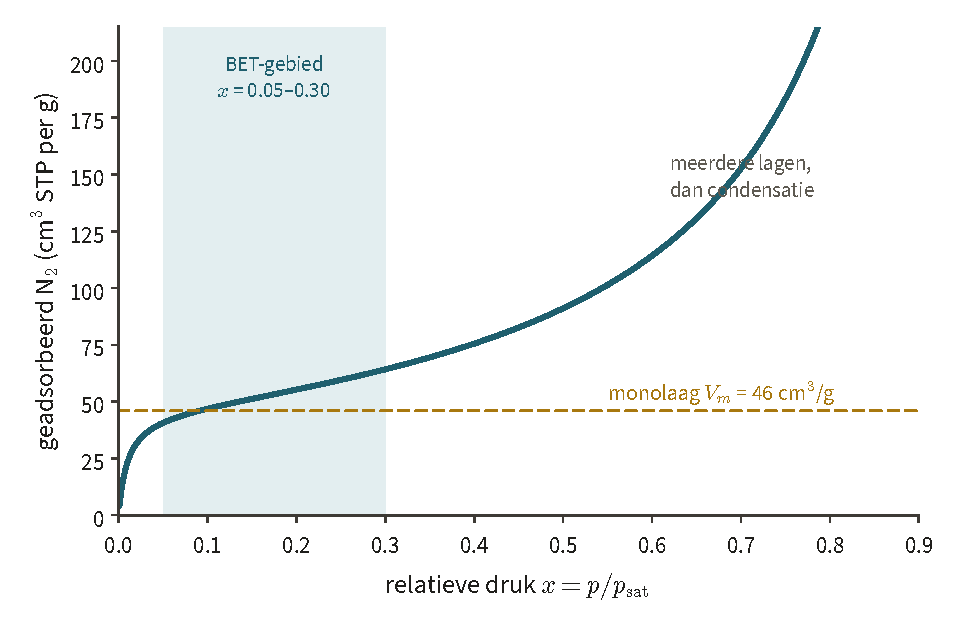
\includegraphics[width=0.7\linewidth]{Figuren/bet_isotherm}
    \caption{Stikstofadsorptie bij \SI{77}{\kelvin} op een poreuze drager (BET-model met $C = 100$ en $V_m = \SI{46}{\centi\metre\cubed\per\gram}$). Rond $x \approx 0.1$ is de eerste laag vol; daarna groeien meer lagen en volgt capillaire condensatie in de poriën.}
    \label{fig:bet-isotherm}
\end{figure}

\begin{voorbeeld}{Het oppervlak van de katalysatordrager}
Voor de $\gamma$-$\mathrm{Al_2O_3}$-korrel van de centrale case levert de BET-rechte $V_m = \SI{46}{\centi\metre\cubed}$ (STP) per gram. Met vergelijking~\eqref{eq:bet-oppervlak}: $a_s = 46 \times 4.35 = \SI{200}{\metre\squared\per\gram}$. Een korrel van \SI{1}{\gram} heeft dus een inwendig oppervlak van \SI{200}{\metre\squared}, terwijl de buitenkant van die korrel nog geen \SI{5}{\centi\metre\squared} meet. Vergelijk met vergelijking~\eqref{eq:specifiek-oppervlak}: zonder poriën zouden de korrels kleiner dan \SI{10}{\nano\metre} moeten zijn.
\end{voorbeeld}

\subsection{Adsorptie uit een oplossing}
\label{sec:adsorptie-oplossing}

Ook opgeloste stoffen adsorberen: kleurstoffen, pesticiden of geurstoffen op actieve kool, eiwitten op een membraan. Het adsorbens is dan zelden homogeen genoeg voor Langmuir, en men gebruikt vaak de empirische \emph{Freundlich-isotherme}
\begin{equation}
q = K_F\,c^{1/n},
\label{eq:freundlich}
\end{equation}
met $q$ de geadsorbeerde hoeveelheid per kg adsorbens, $c$ de concentratie in oplossing en $n > 1$. Op een log--logschaal is dat een rechte. Zoals bij gasadsorptie geldt: hydrofobe, slecht oplosbare moleculen adsorberen het sterkst op hydrofobe kool (hoofdstuk~\ref{ch:intermoleculair}, \S~\ref{sec:im-toepassingen}).

\section{Surfactanten en micelvorming}
\label{sec:surfactanten}

\emph{Surfactanten} (oppervlakte-actieve stoffen) zijn moleculen met een dualistische structuur: een hydrofiele kop en een hydrofobe staart. In water accumuleren zij aan het vloeistof--luchtgrensvlak, met de hydrofobe staart naar de lucht gericht. Hierdoor wordt de oppervlaktespanning sterk verlaagd.

\subsection{De kritische micelconcentratie (CMC)}

Boven een bepaalde concentratie, de \emph{kritische micelconcentratie} (CMC), organiseren surfactanten zich spontaan in aggregaten: \emph{micellen}. In een micel zijn de hydrofobe staarten naar binnen gericht en de hydrofiele koppen naar buiten, zodat het micel als geheel wateroplosbaar is. Onder de CMC gedragen surfactanten zich als gewone opgeloste stoffen; boven de CMC blijft de concentratie vrije surfactant constant en worden bijkomende moleculen in micellen opgenomen.

\begin{voorbeeld}{CMC van natriumdodecylsulfaat}
Natriumdodecylsulfaat (SDS, $\mathrm{CH_3(CH_2)_{11}OSO_3Na}$) heeft een CMC van \SI{8.2e-3}{\mole\per\litre} bij \SI{25}{\celsius}. Onder deze concentratie daalt de oppervlaktespanning geleidelijk met de SDS-concentratie; boven de CMC blijft de oppervlaktespanning constant op ongeveer \SI{35}{\milli\newton\per\metre}. Dit is een direct gevolg van de micelvorming: bijkomende SDS verhoogt enkel het aantal micellen, niet de concentratie vrije surfactant.
\end{voorbeeld}

\subsection{Thermodynamica van micelvorming}

Micelvorming is een spontaan proces met een negatieve Gibbs-energie. De drijvende kracht is de entropie: de waterstructuur rond de hydrofobe staarten (``ijskragen'') wordt verbroken wanneer de staarten zich in een micel samenpakken. Dit \emph{hydrofoob effect} is entropisch van aard, een directe illustratie van de principes uit hoofdstuk~\ref{ch:spontaniteit} (\S~\ref{sec:waarschijnlijkheid-entropie}).

\begin{toepassing}{Tweede case: hoe een wasmiddel vet verwijdert}
Een vetvlek op katoen is hydrofoob en bevochtigt het water slecht. Surfactanten in het wasmiddel adsorberen met hun staart aan het vet en met hun kop naar het water: de grensvlakspanning vet--water daalt van ongeveer \SI{50}{\milli\newton\per\metre} tot enkele \si{\milli\newton\per\metre}. Daardoor verandert de contacthoek (vergelijking~\eqref{eq:young}) en rolt het vet op tot druppeltjes die loskomen van de vezel. Boven de CMC worden die druppeltjes in micellen opgenomen; de geladen koppen houden ze uit elkaar (\S~\ref{sec:colloiden}). Warmer water helpt, omdat vet vloeibaarder wordt en de oppervlaktespanning daalt, maar moderne enzymen en surfactanten werken al bij \SI{30}{\celsius}, wat veel energie bespaart.
\end{toepassing}

\section{Collo\"idale dispersies en stabiliteit}
\label{sec:colloiden}

Een \emph{collo\"ide} is een dispersie van deeltjes met een grootte tussen \SI{1}{\nano\metre} en \SI{1}{\micro\metre} in een continue fase. Voorbeelden: emulsies (melk, mayonaise), suspensies (verf), schuimen (bier), aerosolen (mist). Collo\"idale deeltjes zijn groot genoeg om Brownse beweging te vertonen, maar klein genoeg om niet snel te sedimenteren.

\subsection{Het potentieel van DLVO}
\label{sec:dlvo}

De stabiliteit van een collo\"idale dispersie wordt bepaald door de balans tussen twee krachten:
\begin{itemize}
\item \textbf{Van der Waals-aantrekking} (hoofdstuk~\ref{ch:intermoleculair}): brengt deeltjes samen en leidt tot coagulatie.
\item \textbf{Elektrostatische afstoting}: ontstaat door geladen oppervlakken met een elektrische dubbellaag; werkt de aantrekking tegen.
\end{itemize}
De som van beide krachten als functie van de afstand vormt de \emph{potenti\"ele energiecurve} van DLVO (Derjaguin--Landau--Verwey--Overbeek). Bij voldoende afstoting ontstaat een energiedrempel die coagulatie verhindert; de dispersie is dan kinetisch stabiel (figuur~\ref{fig:dlvo}). Voegt men zout toe, dan wordt de afstoting korter van bereik en verdwijnt de drempel.

\begin{figure}[htb]
    \centering
    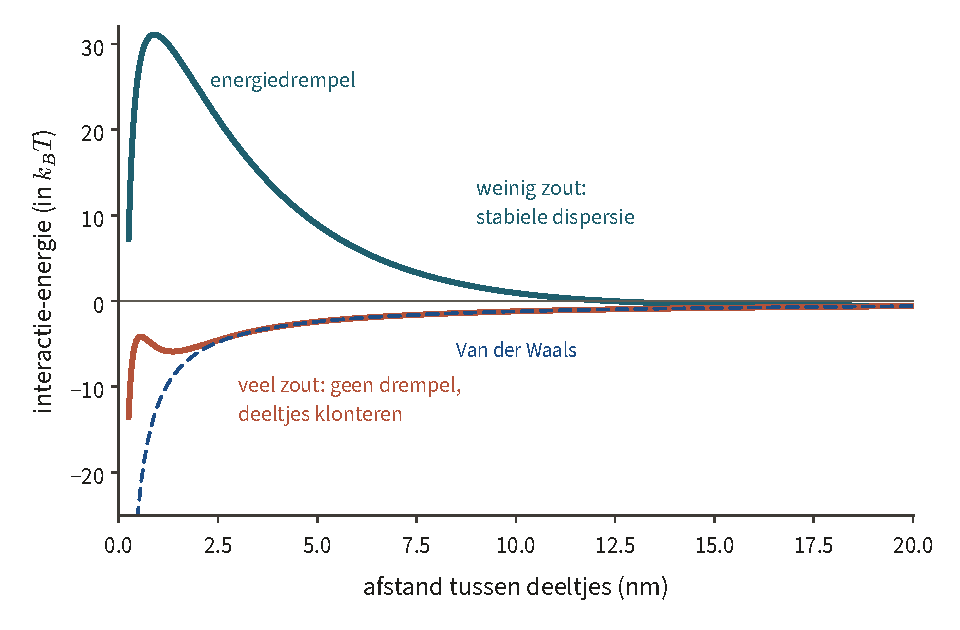
\includegraphics[width=0.7\linewidth]{Figuren/dlvo}
    \caption{DLVO-energie tussen twee colloïdale deeltjes (schematisch): de som van een Van der Waals-aantrekking en een elektrostatische afstoting. Bij weinig zout is er een drempel van tientallen $k_BT$ en blijft de dispersie stabiel; bij veel zout verdwijnt de drempel en klonteren de deeltjes samen.}
    \label{fig:dlvo}
\end{figure}

\subsection{De elektrische dubbellaag}

In waterige oplossingen krijgen collo\"idale deeltjes een oppervlaktelading door ionisatie van oppervlaktegroepen, adsorptie van ionen (\S~\ref{sec:adsorptie-grensvlakken}) of isomorfe substitutie. Deze lading wordt gecompenseerd door een tegenionenwolk: de \emph{elektrische dubbellaag}. Het model van Gouy--Chapman--Stern beschrijft twee gebieden:
\begin{enumerate}
\item Een \emph{Stern-laag}: stevig gebonden tegenionen dicht bij het oppervlak.
\item Een \emph{diffuse laag}: een wolk van tegenionen met geleidelijk afnemende concentratie, die in de bulk overgaat.
\end{enumerate}
Het potentiaalverloop in de diffuse laag is exponentieel, met karakteristieke lengte $\kappa^{-1}$ (Debye-lengte). In water bij \SI{25}{\celsius} geldt voor een 1:1-zout $\kappa^{-1} \approx \SI{0.304}{\nano\metre}/\sqrt{c/(\si{\mole\per\litre})}$: ongeveer \SI{10}{\nano\metre} in zoet water ($c \approx \SI{1}{\milli\mole\per\litre}$), maar slechts \SI{0.4}{\nano\metre} in zeewater. Dat verklaart waarom rivierslib neerslaat zodra de rivier de zee bereikt: de delta's van de Schelde en de Nijl zijn ook een colloïdchemisch verschijnsel.

\subsection{De zeta-potentiaal}

Het praktisch meetbare potentiaal aan de grens tussen de Stern-laag en de diffuse laag is de \emph{zeta-potentiaal} $\zeta$. Een collo\"ide met $|\zeta| > \SI{30}{\milli\volt}$ is doorgaans stabiel; bij $|\zeta| < \SI{10}{\milli\volt}$ coaguleert de dispersie snel.

\begin{voorbeeld}{Zeta-potentiaal en waterzuivering}
In waterzuiveringsinstallaties worden collo\"idale deeltjes (klei, organisch materiaal) verwijderd door coagulatie. Door toevoeging van $\mathrm{Al_2(SO_4)_3}$ of $\mathrm{FeCl_3}$ wordt de zeta-potentiaal verlaagd: de veelwaardige kationen ($\mathrm{Al^{3+}}$, $\mathrm{Fe^{3+}}$) comprimeren de dubbellaag en reduceren $\zeta$. Hierdoor verliest het collo\"ide zijn stabiliteit en slaat het neer. Dit is het werkingsmechanisme van flocculatie in drinkwaterproductie.
\end{voorbeeld}

\subsection{Elektrokinetische verschijnselen}

Wanneer een collo\"ide met geladen oppervlak zich in een elektrisch veld bevindt, kunnen twee verschijnselen optreden:
\begin{itemize}
\item \textbf{Elektroforese}: de deeltjes bewegen naar de tegengesteld geladen elektrode.
\item \textbf{Elektro-osmose}: de vloeistof beweegt langs een geladen vaste wand wanneer een elektrisch veld wordt aangelegd.
\end{itemize}
Beide verschijnselen worden beschreven door de vergelijking van Smoluchowski en worden toegepast in inktprinters, elektroforetische coatings, DNA-scheiding en microfluidica.

\section{Emulsies en stabilisatoren}
\label{sec:emulsies}

Een \emph{emulsie} is een dispersie van een vloeistof in een andere onmengbare vloeistof. Twee types worden onderscheiden:
\begin{itemize}
\item \textbf{Olie-in-water (O/W)}: oliedruppels in waterige fase (melk, mayonaise, cosmeticum).
\item \textbf{Water-in-olie (W/O)}: waterdruppels in oliefase (boter, margarine, sommige zalven).
\end{itemize}
Emulsies zijn thermodynamisch onstabiel (de Gibbs-energie van de grensvlakken is positief), maar kunnen kinetisch stabiel worden gemaakt door \emph{emulgatoren}: surfactanten of vaste deeltjes die zich aan het vloeistof--vloeistofgrensvlak hechten en een beschermende laag vormen.

\subsection{Het HLB-getal}

De keuze van de juiste surfactant voor een emulsie wordt geholpen door het \emph{HLB-getal} (Hydrofiel--Lipofiel Balans):
\begin{itemize}
\item HLB 3--6: W/O-emulgator.
\item HLB 8--18: O/W-emulgator.
\end{itemize}
Voor mayonaise (O/W) gebruikt men bijvoorbeeld eiwit (HLB $\sim$ 13); voor margarine (W/O) gebruikt men mono- en diglyceriden (HLB $\sim$ 4).

\section{Schuimen en antischuimmiddelen}

Een \emph{schuim} is een dispersie van gas in vloeistof. Schuimen zijn kinetisch stabiel door surfactanten die de gasbel-wanden versterken (Marangoni-effect: herstel van lokale oppervlaktespanningsgradi\"enten). Schuimen zijn gewenst in bier, scheerschuim en brandblusschuim, maar ongewenst in fermentoren, destillatiekolommen en waswater.

\emph{Antischuimmiddelen} werken door de lokale oppervlaktespanning sterk te verlagen of door de film te verzwakken. Vaak gebruikt men siliconenoli\"e\"en of hydrofoob silica.

\section{De vaste stof: van atomen naar kristallen}
\label{sec:vaste-stof}

Het oppervlak waarop alles in dit hoofdstuk gebeurt, hoort bij een vaste stof. Een katalysatordrager, een elektrode, een pigment of een zeoliet heeft eigenschappen die rechtstreeks volgen uit hoe de atomen gerangschikt zijn: in een regelmatig kristal, met defecten, of amorf. Voor de chemisch ingenieur is de vaste stof dus veel meer dan een passieve drager: de kristalstructuur bepaalt de katalytische activiteit, de elektronenstructuur ligt aan de basis van zonnecellen en led's, en defecten bepalen de sterkte en de corrosie van constructiematerialen.

\subsection{Kristalstructuren: de Bravais-roosters}
\label{sec:bravais}

Een \emph{kristal} is een vaste stof waarin de atomen in een regelmatige, driedimensionale rangschikking zijn geordend. Deze rangschikking wordt beschreven door een \emph{kristalrooster}: een oneindige herhaling van een elementaire cel langs drie onafhankelijke richtingen.

\subsubsection{De elementaire cel}

De \emph{elementaire cel} is de kleinste eenheid die, door herhaling in drie richtingen, het volledige kristal opbouwt. Zij wordt gekenmerkt door drie roosterconstanten $a$, $b$, $c$ (lengtes) en drie hoeken $\alpha$, $\beta$, $\gamma$ (tussen de assen).

Er bestaan precies \emph{14} onafhankelijke roostertypes, de \emph{Bravais-roosters}, verdeeld over 7 kristalsystemen:
\begin{itemize}
\item \textbf{Kubisch}: primitief (P), ruimtelijk gecentreerd (I), vlakgecentreerd (F).
\item \textbf{Tetragonaal}: primitief, ruimtelijk gecentreerd.
\item \textbf{Orthorombisch}: primitief, ruimtelijk gecentreerd, vlakgecentreerd, basaal gecentreerd.
\item \textbf{Hexagonaal}: primitief.
\item \textbf{Trigonaal} (rhombohedrisch): primitief.
\item \textbf{Monoclien}: primitief, basaal gecentreerd.
\item \textbf{Triklien}: primitief.
\end{itemize}
Tel je deze op (3+2+4+1+1+2+1), dan kom je inderdaad op precies 14 uit: geen enkel ander roostertype is met een periodieke driedimensionale rangschikking van punten verenigbaar.

\subsubsection{De drie kubische roosters}

De eenvoudigste en belangrijkste roosters voor metallische en ionische vaste stoffen zijn de drie kubische types:

\begin{itemize}
\item \textbf{Primitief kubisch (P)}: atomen op de 8 hoeken van een kubus. Aantal atomen per cel: $8 \times \tfrac{1}{8} = 1$.
\item \textbf{Ruimtelijk gecentreerd kubisch (BCC, I)}: bijkomend atoom in het centrum. Aantal atomen per cel: $1 + 1 = 2$.
\item \textbf{Vlakgecentreerd kubisch (FCC, F)}: bijkomend atoom op elk van de 6 vlakken (gedeeld door 2 cellen). Aantal atomen per cel: $1 + 6 \times \tfrac{1}{2} = 4$.
\end{itemize}

\begin{figure}[htb]
    \centering
    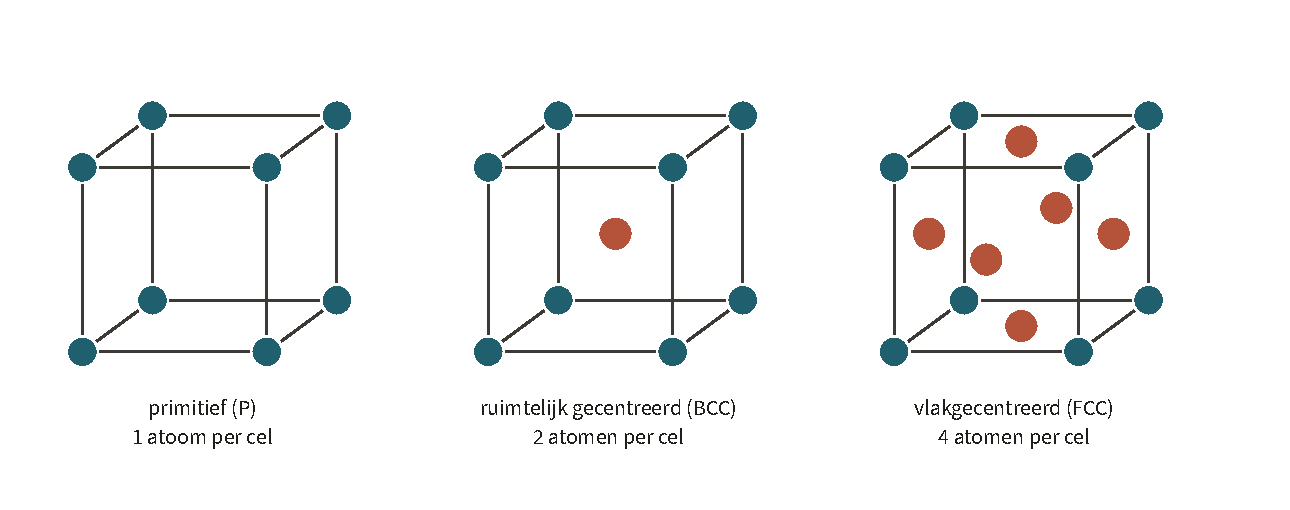
\includegraphics[width=0.95\linewidth]{Figuren/kubische_roosters}
    \caption{De drie kubische Bravais-roosters: primitief kubisch (enkel hoekatomen), ruimtelijk gecentreerd (BCC, met een atoom in het centrum) en vlakgecentreerd (FCC, met een atoom op elk van de zes vlakken). Een hoekatoom wordt gedeeld door acht cellen, een vlakatoom door twee.}
    \label{fig:kubische-roosters}
\end{figure}

\begin{voorbeeld}{Pakking en atoomradius in FCC}
In een FCC-rooster (bv. Cu, Al, $\gamma$-Fe) raken de atomen langs de diagonaal van een vlak. Met roosterconstante $a$ geldt $4r = a\sqrt{2}$, zodat $r = a\sqrt{2}/4$. Voor koper met $a = \SI{0.361}{\nano\metre}$:
\[
r = \frac{\SI{0.361}{\nano\metre}\,\sqrt{2}}{4} = \SI{0.128}{\nano\metre}.
\]
De pakking (fractie van het volume ingenomen door atomen) bedraagt $\pi/(3\sqrt{2}) \approx 0.74$ --- de dichtst mogelijke bolpakking.
\end{voorbeeld}

\subsubsection{Structuren van ionische en covalente vaste stoffen}

Enkele veelvoorkomende structuurtypen:

\begin{itemize}
\item \textbf{NaCl-structuur}: FCC-rooster van $\mathrm{Cl^-}$ met $\mathrm{Na^+}$ in alle octa\"edrische holtes. Co\"ordinatiegetal 6:6.
\item \textbf{CsCl-structuur}: primitief kubisch rooster van $\mathrm{Cl^-}$ met $\mathrm{Cs^+}$ in het lichaam-centrum. Co\"ordinatiegetal 8:8.
\item \textbf{Zinkblende (ZnS)}: FCC-rooster van $\mathrm{S^{2-}}$ met $\mathrm{Zn^{2+}}$ in de helft van de tetra\"edrische holtes. Co\"ordinatie 4:4. Belangrijk voor halfgeleiders (GaAs, CdTe).
\item \textbf{Fluoriet ($\mathrm{CaF_2}$)}: FCC-rooster van $\mathrm{Ca^{2+}}$ met $\mathrm{F^-}$ in alle tetra\"edrische holtes. Belangrijk voor $\mathrm{UO_2}$, $\mathrm{CeO_2}$, $\mathrm{ZrO_2}$.
\item \textbf{Diamant}: FCC-rooster met twee interpenetrerende subroosters, elk atoom tetra\"edrisch omringd. Dit is de structuur van Si, Ge, C (diamant).
\end{itemize}

\subsection{R\"ontgendiffractie en de wet van Bragg}
\label{sec:xrd}

De experimentele methode bij uitstek voor de bepaling van kristalstructuren is \emph{r\"ontgendiffractie} (XRD). De golflengte van r\"ontgenstraling (\SIrange{0.1}{1}{\angstrom}) is van dezelfde orde als interatomaire afstanden, zodat diffractie optreedt aan de roostervlakken.

\subsubsection{Millerindices: het aanduiden van roostervlakken}
\label{sec:miller}

Om een specifieke set evenwijdige roostervlakken ondubbelzinnig aan te duiden, gebruikt men \emph{Millerindices} $(hkl)$: drie gehele getallen, bepaald door de omgekeerde waarden van de snijpunten van het vlak met de drie kristalassen (uitgedrukt in eenheden van de roosterconstanten $a$, $b$, $c$) te nemen en tot de kleinste gehele verhouding te herleiden. Een vlak dat de $x$-, $y$- en $z$-as elk op afstand $a$ snijdt, heeft dus Millerindices $(111)$; een vlak evenwijdig met de $y$- en $z$-as (het snijdt enkel de $x$-as) heeft indices $(100)$.

Voor een \emph{kubisch} rooster met roosterconstante $a$ is de afstand tussen opeenvolgende $(hkl)$-vlakken:
\begin{equation}
\boxed{\;d_{hkl} = \frac{a}{\sqrt{h^2+k^2+l^2}}.\;}
\label{eq:dhkl}
\end{equation}
Voor de $(111)$-vlakken geeft dit bijvoorbeeld $d_{111}=a/\sqrt{1^2+1^2+1^2}=a/\sqrt3$ --- de relatie die we hieronder gebruiken om, via de wet van Bragg, de roosterconstante van koper te bepalen. Deze combinatie --- Millerindices om een vlak te identificeren, vergelijking~\eqref{eq:dhkl} om de bijhorende vlakafstand te berekenen, en de wet van Bragg (hieronder) om die vlakafstand experimenteel te meten --- vormt samen het volledige gereedschap om een onbekende kubische kristalstructuur te karakteriseren.

\subsubsection{De wet van Bragg}
\label{sec:bragg}

Wanneer een r\"ontgenbundel invalt op een kristal onder hoek $\theta$ ten opzichte van een set roostervlakken met intervlakafstand $d$, treden versterkende interferenties op wanneer:
\begin{equation}
\boxed{\;n\lambda = 2\,d\,\sin\theta\;}
\label{eq:bragg}
\end{equation}
waarin $\lambda$ de golflengte en $n$ een geheel getal is (de ``orde''). Uit de gemeten hoeken $\theta$ kan $d$ worden berekend via vergelijking~\eqref{eq:dhkl}, en uit het volledige diffractiepatroon de kristalstructuur worden gereconstrueerd.

\begin{figure}[htb]
    \centering
    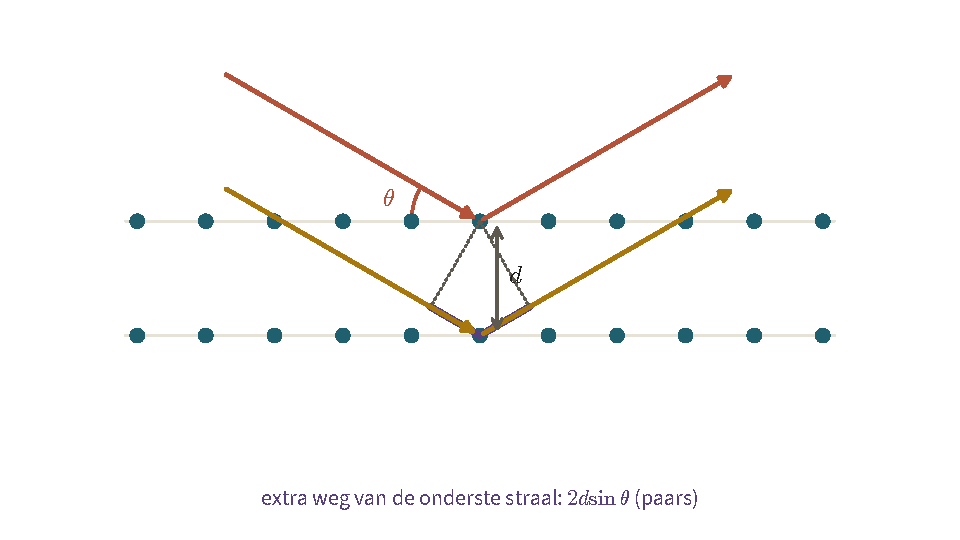
\includegraphics[width=0.75\linewidth]{Figuren/bragg_geometrie}
    \caption{Braggdiffractie aan twee evenwijdige roostervlakken op afstand $d$. De straal die het onderste vlak treft, legt een extra weg $2d\sin\theta$ af. Enkel als dat een geheel aantal golflengten is, versterken de gereflecteerde stralen elkaar (vergelijking~\eqref{eq:bragg}).}
    \label{fig:bragg-geometrie}
\end{figure}

\begin{voorbeeld}{Bepaling van de roosterconstante van koper --- let op $2\theta$ versus $\theta$}
Een veelvoorkomende valkuil bij het praktisch gebruik van de wet van Bragg is de volgende: XRD-toestellen rapporteren doorgaans de hoek $2\theta$ tussen de invallende en de gediffracteerde bundel (de hoek waarover de detector effectief draait), \emph{niet} de hoek $\theta$ uit vergelijking~\eqref{eq:bragg} zelf, die ten opzichte van het roostervlak wordt gemeten. Het rechtstreeks invullen van een gerapporteerde $2\theta$-waarde als $\theta$ levert een systematisch verkeerd resultaat op.

Een poederdiffractiepatroon van koper ($\lambda = \SI{0.154}{\nano\metre}$, Cu K$\alpha$) toont een eerste piek bij $2\theta = 43.1^\circ$, dus $\theta = 21.55^\circ$. Voor de $(111)$-vlakken geeft de wet van Bragg ($n=1$):
\[
d_{111} = \frac{\lambda}{2\sin\theta} = \frac{\SI{0.154}{\nano\metre}}{2\sin(21.55^\circ)} = \frac{\SI{0.154}{\nano\metre}}{0.7337} \approx \SI{0.210}{\nano\metre}.
\]
Met vergelijking~\eqref{eq:dhkl}, $d_{111} = a/\sqrt{3}$ voor een kubisch rooster:
\[
a = d_{111}\sqrt{3} \approx (\SI{0.210}{\nano\metre})(1.732) \approx \SI{0.363}{\nano\metre},
\]
in uitstekende overeenstemming met de bekende roosterconstante van Cu ($a=\SI{0.3615}{\nano\metre}$, reeds gebruikt in \S~\ref{sec:bravais}). Zou men $43.1^\circ$ ten onrechte rechtstreeks als $\theta$ hebben ingevuld, dan volgt $d_{111}\approx\SI{0.113}{\nano\metre}$ en $a\approx\SI{0.195}{\nano\metre}$ --- bijna een factor twee te klein, en duidelijk onverenigbaar met de bekende dichtheid en atoomstraal van koper. Controleer daarom bij elke XRD-analyse expliciet of de gerapporteerde hoek $\theta$ dan wel $2\theta$ voorstelt, vooraleer de wet van Bragg toe te passen.
\end{voorbeeld}

\subsubsection{Het poederdiffractiepatroon}

In plaats van een enkelkristal wordt in de praktijk vaak een poeder gebruikt, zodat alle mogelijke vlakori\"entaties simultaan aanwezig zijn. Het resulterende \emph{poederdiffractiepatroon} (XRD-patroon) is een reeks pieken bij verschillende $2\theta$. De positie van de pieken geeft de roosterconstanten; de intensiteit geeft de atoomposities binnen de cel; de breedte geeft informatie over korrelgrootte en defecten.

\begin{figure}[htb]
    \centering
    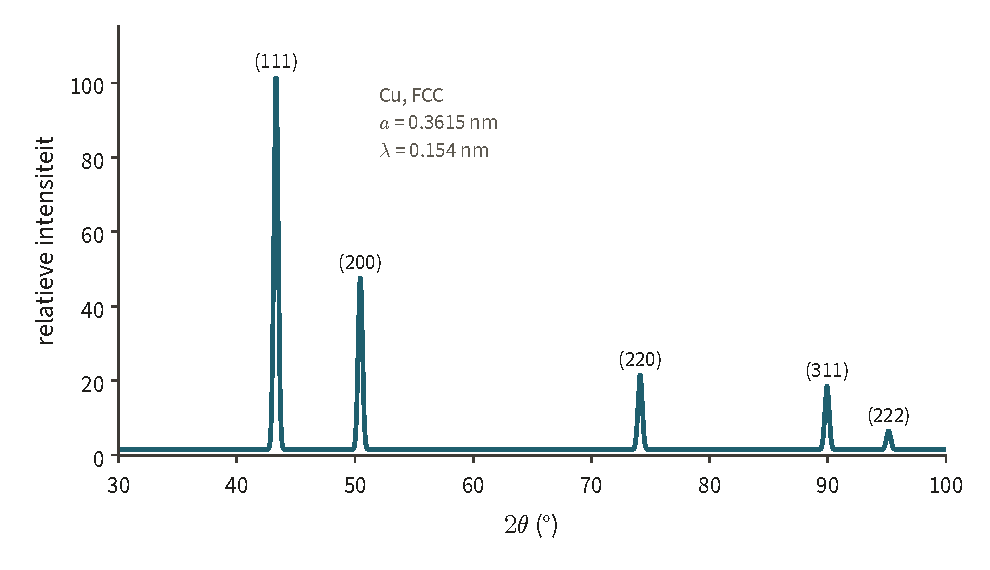
\includegraphics[width=0.75\linewidth]{Figuren/xrd_poederpatroon}
    \caption{Berekend poederdiffractogram van koper (FCC, $a = \SI{0.3615}{\nano\metre}$, Cu K$\alpha$-straling). In een FCC-rooster zijn enkel reflecties zichtbaar waarvoor $h$, $k$ en $l$ allemaal even of allemaal oneven zijn. Elke piekpositie geeft via de wet van Bragg en vergelijking~\eqref{eq:dhkl} de roosterconstante.}
    \label{fig:xrd-poederpatroon}
\end{figure}

Vergelijking met databanken (JCPDS, ICDD) laat toe een onbekende stof in seconden te identificeren. Dit is standaard in katalysatorkarakterisatie, kwaliteitscontrole, forensische chemie en farmaceutische analyse (polymorfie).

Ook de \emph{breedte} van een piek is nuttig. Een oneindig groot kristal geeft een scherpe piek; een kristalletje van enkele nanometer heeft te weinig roostervlakken om buiten de Braggvoorwaarde volledig uit te doven, en geeft een brede piek. De \emph{vergelijking van Scherrer} schat de kristalgrootte $\tau$:
\begin{equation}
\tau = \frac{K\lambda}{\beta\cos\theta},
\label{eq:scherrer}
\end{equation}
met $K \approx 0.9$ en $\beta$ de piekbreedte op halve hoogte, in radialen op de $2\theta$-schaal.

\begin{voorbeeld}{Hoe groot zijn de platinadeeltjes op de katalysator?}
Het diffractogram van de katalysator uit de centrale case toont een brede Pt(111)-piek bij $2\theta = 39.8^\circ$ met een halfwaardebreedte van $4.5^\circ = \SI{0.0785}{\radian}$. Met $\theta = 19.9^\circ$:
\[
\tau = \frac{(0.9)(\SI{0.154}{\nano\metre})}{(0.0785)\cos 19.9^\circ} = \SI{1.9}{\nano\metre}.
\]
De platinadeeltjes zijn dus ongeveer \SI{2}{\nano\metre} groot: goed verdeeld. Na een tijd bij hoge temperatuur wordt de piek smaller; de deeltjes groeien samen (sinteren) en de katalysator verliest actief oppervlak. XRD is zo een snelle controle op de veroudering van een katalysator.
\end{voorbeeld}

\subsection{Defecten in kristallen}
\label{sec:defecten}

Een perfect kristal zonder defecten bestaat in de praktijk niet. Zelfs de zuiverste materialen bevatten defecten, en deze defecten bepalen vaak de macroscopische eigenschappen: elektrische geleiding, mechanische sterkte, kleur, katalytische activiteit. Defecten worden ingedeeld naar dimensie.

\subsubsection{Puntdefecten}

\begin{itemize}
\item \textbf{Vacatures}: een ontbrekend atoom op een roosterplaats. Evenwichtsvacatures volgen $\exp(-E_v/k_BT)$, met $E_v \sim \SI{1}{\electronvolt}$ in metalen. Bij \SI{300}{\kelvin} is deze fractie volledig verwaarloosbaar ($\sim10^{-17}$): pas dicht bij het smeltpunt (bijvoorbeeld \SI{1300}{\kelvin} voor koper, smeltpunt \SI{1358}{\kelvin}) wordt de vacaturefractie praktisch relevant, met een typische waarde van $\sim10^{-4}$ --- een gevolg van de sterke exponenti\"ele temperatuursafhankelijkheid, geheel analoog aan de Arrhenius-gevoeligheid van reactiesnelheden (hoofdstuk~\ref{ch:kinetiek}).
\item \textbf{Interstiti\"eel}: een extra atoom op een niet-roosterplaats. Vaak in combinatie met vacatures (Frenkel-defect in ionische kristallen).
\item \textbf{Onzuiverheden (doping)}: een vreemd atoom op een roosterplaats. Cruciaal voor halfgeleiders (hoofdstuk~\ref{ch:kwantum} en \S~\ref{sec:doping}) en katalysatoren (hoofdstuk~\ref{ch:kinetiek}).
\item \textbf{Schottky-defect}: een koppel vacatures in ionische kristallen (een kation- en een anionvacature), zodat neutraliteit behouden blijft.
\end{itemize}

\subsubsection{Lijndefecten (dislocaties)}

\emph{Dislocaties} zijn \'e\'endimensionale defecten die plastische vervorming mogelijk maken. De twee belangrijkste types:
\begin{itemize}
\item \textbf{Randdislocatie (edge)}: een extra half-vlak ingevoerd in het kristal.
\item \textbf{Schroefdislocatie (screw)}: het rooster is langs een as verschoven.
\end{itemize}
Dislocaties bepalen de hardheid, rekeigenschappen en \emph{kruip} van metalen. In katalysatoren zijn schroefdislocaties vaak actieve sites, omdat atomen aan het oppervlak daar zwakker gebonden zijn.

\subsubsection{Vlakdefecten}

\begin{itemize}
\item \textbf{Korrelgrenzen}: grenzen tussen kristallieten in polykristallijne materialen. Be\"invloeden diffusie, corrosie en elektrische geleiding.
\item \textbf{Stacking faults}: fout in de stapelvolgorde van atoomvlakken.
\item \textbf{Antifase-grenzen}: in geordende legeringen.
\end{itemize}

\subsubsection{Non-stoichiometrie}

Vele vaste stoffen wijken af van de ideale stoichiometrie. \emph{Non-stoichiometrische verbindingen} hebben een variabele samenstelling, zoals $\mathrm{Fe_{1-x}O}$ (wustiet, $x \sim 0.05$), $\mathrm{TiO_{2-x}}$, $\mathrm{UO_{2+x}}$. De oorzaak is een combinatie van vacatures en geoxideerde/gereduceerde ionen. Non-stoichiometrie is cruciaal voor katalysatoren (bv. $\mathrm{V_2O_{5-x}}$ in het contactproces, hoofdstuk~\ref{ch:kinetiek}) en voor batterijmaterialen (Li-ion-intercalatie).

\subsection{Elektronenstructuur: van ge\"isoleerd atoom tot vaste stof}

In hoofdstuk~\ref{ch:kwantum} zagen we dat een ge\"isoleerd atoom discrete energieniveaus heeft. Wanneer $N$ atomen samengebracht worden in een kristal, overlappen hun golffuncties. Volgens het uitsluitingsprincipe van Pauli (hoofdstuk~\ref{ch:kwantum}) mogen geen twee elektronen dezelfde toestand bezetten. Hierdoor splitst elk niveau van het ge\"isoleerde atoom in $N$ niveaus, dicht opeen. Het is hetzelfde mechanisme als bij de molecuulorbitalen van hoofdstuk~\ref{ch:kwantum} (\S~\ref{sec:molecuulorbitalen}): twee atoomorbitalen geven een bindend en een antibindend niveau, $N$ atoomorbitalen geven er $N$. Voor macroscopisch $N$ ($\sim10^{23}$) vormen deze niveaus een continu\"um: een \emph{energieband}.

\subsubsection{Geleiders, halfgeleiders en isolatoren}

In een kristal worden twee banden onderscheiden:
\begin{itemize}
\item \textbf{Valentieband}: de hoogste geheel gevulde band.
\item \textbf{Geleidingsband}: de eerstvolgende, lege of deels gevulde band.
\end{itemize}
Tussen beide kan een \emph{verboden zone} (band gap, $E_g$) liggen. De classificatie:
\begin{itemize}
\item \textbf{Geleider} (metaal): de valentieband is deels gevuld of overlapt met de geleidingsband. Elektronen kunnen vrij bewegen; $E_g = 0$.
\item \textbf{Halfgeleider}: $E_g = \SIrange{0.5}{3}{\electronvolt}$. Bij lage temperatuur is de geleidingsband leeg (geen geleiding); bij hoge temperatuur kunnen elektronen thermisch worden geactiveerd.
\item \textbf{Isolator}: $E_g > \SI{4}{\electronvolt}$. De thermische activering is verwaarloosbaar bij kamertemperatuur.
\end{itemize}

\begin{voorbeeld}{Band gaps van enkele materialen}
\begin{itemize}
\item Si: $E_g = \SI{1.12}{\electronvolt}$ (halfgeleider).
\item GaAs: $E_g = \SI{1.42}{\electronvolt}$ (halfgeleider).
\item Diamant: $E_g \approx \SI{5.5}{\electronvolt}$ (isolator).
\item $\mathrm{SiO_2}$: $E_g \approx \SI{9}{\electronvolt}$ (isolator).
\item Cu: $E_g = 0$ (geleider).
\end{itemize}
Het verschil tussen Si en GaAs is klein maar cruciaal: GaAs laat hogere snelheden en zonnecellen met hogere effici\"entie toe, Si domineert de markt via lagere kostprijs.
\end{voorbeeld}

\subsubsection{Doping van halfgeleiders}
\label{sec:doping}

Door kleine hoeveelheden onzuiverheden toe te voegen (\emph{doping}) kan de geleidingsband bevolkt worden:
\begin{itemize}
\item \textbf{n-type}: donoratomen (bv. P in Si, 5 valentie-elektronen) leveren een extra elektron. Donorniveau vlak onder de geleidingsband.
\item \textbf{p-type}: acceptoratomen (bv. B in Si, 3 valentie-elektronen) cre\"eren een gat. Acceptorniveau vlak boven de valentieband.
\end{itemize}
De benodigde activeringsenergie om deze donor- of acceptorniveaus te ioniseren is nu veel kleiner dan $E_g$, zodat reeds bij kamertemperatuur voldoende ladingsdragers beschikbaar zijn. Doping is de basis van transistors, zonnecellen, LED's en batterijbesturing.

\subsection{Thermodynamica van vaste stoffen}

De thermodynamica uit hoofdstuk~\ref{ch:spontaniteit} is volledig van toepassing op vaste stoffen. Enkele bijzondere aspecten:

\subsubsection{Faseovergangen in de vaste stof}

Naast smelten en verdampen kent de vaste stof ook \emph{vast-vast faseovergangen}. IJzer transformeert bij \SI{912}{\celsius} van BCC ($\alpha$-Fe) naar FCC ($\gamma$-Fe), en bij \SI{1394}{\celsius} terug naar BCC ($\delta$-Fe). Koolstof kent grafiet (stabiel bij 1 bar) en diamant (stabiel bij hoge druk). De Clapeyron-vergelijking uit hoofdstuk~\ref{ch:niet-reagerend} is van toepassing, maar de volumeveranderingen in de vaste fase zijn klein.

\subsubsection{Smeltentropie en -enthalpie}

Smeltenthalpie\"en van metalen volgen de regel van Richards: $\Delta S_{\text{fus}} \approx \SI{8.4}{\joule\per\mole\per\kelvin}$ voor vele metalen. Dit is een empirische schatting die de uniformiteit van smeltprocessen benadrukt.

\subsubsection{Warmtecapaciteit van vaste stoffen}

Bij lage temperatuur volgt $C_V$ de wet van Debye ($T^3$-afhankelijkheid). Bij hoge temperatuur nadert $C_V$ de klassieke limiet van Dulong--Petit:
\begin{equation}
C_{V,m} \approx 3R = \SI{24.9}{\joule\per\mole\per\kelvin}.
\end{equation}
Deze wet is een directe toepassing van het equipartitiebeginsel: elk atoom heeft 6 vrijheidsgraden (3 kinetisch + 3 potentieel), met $\tfrac{1}{2}k_BT$ per vrijheidsgraad.

\begin{voorbeeld}{Warmtecapaciteit van koper en diamant}
Voor Cu bij \SI{298}{\kelvin} geldt $C_{p,m} \approx \SI{24.4}{\joule\per\mole\per\kelvin}$, vrijwel gelijk aan $3R = \SI{24.9}{\joule\per\mole\per\kelvin}$. De overeenkomst met de wet van Dulong--Petit bevestigt dat alle atomaire vrijheidsgraden thermisch actief zijn. Voor diamant bij \SI{298}{\kelvin} geldt $C_{p,m} \approx \SI{6.1}{\joule\per\mole\per\kelvin}$, veel lager dan $3R$, wegens de hoge frequenties van de C--C-bindingen (kwantummechanische bevriezing bij kamertemperatuur, hoofdstuk~\ref{ch:kwantum}, \S~\ref{sec:moleculaire-beweging}).
\end{voorbeeld}

\subsection{Materiaaleigenschappen sturen via defecten}

De ingenieur kan materiaaleigenschappen sturen via \emph{defect engineering}:

\begin{itemize}
\item \textbf{Legering}: door toevoeging van vreemde atomen worden dislocaties verankerd, het materiaal wordt harder (bv. staal = Fe + C + Cr + Mn).
\item \textbf{Doping}: halfgeleiders worden geleidbaar gemaakt via gecontroleerde onzuiverheden (\S~\ref{sec:doping}).
\item \textbf{Korrelgrootte}: volgens Hall--Petch neemt de hardheid toe met $\sim d^{-1/2}$ ($d$ korrelgrootte). Nanokristallijne materialen zijn aanzienlijk harder.
\item \textbf{Warmtebehandeling}: temperatuurverloop regelt de verdeling van defecten en faseverdeling.
\end{itemize}


\section{Toepassingen in de procesindustrie}

\begin{itemize}
\item \textbf{Katalysatoren}: een poreuze drager met groot BET-oppervlak, actieve metaaldeeltjes van enkele nanometer, en een kristalstructuur die de selectiviteit bepaalt (zeolieten). De kinetiek van oppervlaktereacties volgt in hoofdstuk~\ref{ch:kinetiek}.
\item \textbf{Scheiding door adsorptie}: gasdroging met silicagel en zeolieten, PSA voor waterstof, stikstof en zuurstof, actieve kool voor drinkwater en afgassen.
\item \textbf{Wasmiddelen en cosmetica}: surfactanten, micellen, emulsies.
\item \textbf{Waterzuivering}: coagulatie en flocculatie via de zeta-potentiaal, adsorptie op actieve kool.
\item \textbf{Voeding en farmacie}: emulsies (melk, mayonaise, crèmes), schuimen, suspensies, liposomen; polymorfie van geneesmiddelen, gecontroleerd met XRD.
\item \textbf{Mijnbouw}: flotatie, waarbij hydrofoob gemaakte ertsdeeltjes aan luchtbellen hechten.
\item \textbf{Coatings en verf}: bevochtiging, pigmentdispersies, hechting.
\item \textbf{Energie}: halfgeleiders voor zonnecellen en led's, intercalatiematerialen ($\mathrm{LiCoO_2}$, $\mathrm{LiFePO_4}$) voor batterijen, perovskieten voor brandstofcellen (hoofdstuk~\ref{ch:elektrochemie}).
\item \textbf{Constructiematerialen}: staal, roestvast staal, keramiek, beton: polykristallijn, met bewust gestuurde defecten.
\end{itemize}

\section{Samenvatting en reflectie}

Grensvlakken en vaste stoffen brengen bijna alles uit de vorige hoofdstukken samen: de intermoleculaire krachten bepalen oppervlaktespanning en adsorptie, de Gibbsenergie bepaalt of een emulsie stabiel is of een druppel verdampt, en de kwantummechanica bepaalt de banden van een halfgeleider. In het laatste hoofdstuk, over kinetiek, gebruiken we de adsorptie-isothermen om te beschrijven hoe snel een reactie op een katalysatoroppervlak verloopt.

\begin{samenvatting}{Grensvlakken en materialen}
\begin{itemize}
\item Het specifiek oppervlak schaalt met $1/d$; poreuze materialen halen honderden tot duizend \si{\metre\squared\per\gram}.
\item Oppervlaktespanning $\sigma = (\partial G/\partial A)_{T,p}$. Young--Laplace: $\Delta p = 2\sigma/r$. Capillaire stijghoogte $h = 2\sigma\cos\theta/\rho g r$.
\item Young: $\sigma_{sg} = \sigma_{sl} + \sigma_{lg}\cos\theta$; lage oppervlakte-energie geeft slechte bevochtiging.
\item Kelvin: kleine druppels hebben een hogere dampdruk; in nauwe poriën condenseert damp onder $p_\mathrm{sat}$.
\item Fysisorptie (zwak, meerdere lagen) en chemisorptie (chemische binding, \'e\'en laag) zijn exotherm. Langmuir: $\theta = Kp/(1+Kp)$; BET meet het oppervlak met N$_2$ bij \SI{77}{\kelvin}. Adsorbentia laden koud en onder druk, regenereren warm of bij lage druk.
\item Surfactanten verlagen $\sigma$ en vormen micellen boven de CMC. Colloïden zijn kinetisch stabiel door een DLVO-drempel; zout en meerwaardige ionen breken die af.
\item Kristallen: 14 Bravais-roosters; FCC en hcp zijn het dichtst gepakt (\SI{74}{\percent}). XRD: $n\lambda = 2d\sin\theta$ met $d_{hkl} = a/\sqrt{h^2+k^2+l^2}$; piekbreedte geeft de kristalgrootte (Scherrer).
\item Defecten en doping bepalen sterkte, geleidbaarheid en katalytische activiteit. Banden ontstaan uit dezelfde orbitaaloverlap als molecuulorbitalen.
\end{itemize}
\end{samenvatting}

\begin{reflectie}{Grensvlakken en materialen}
\begin{enumerate}
\item Waarom heeft een katalysator met hetzelfde metaalgehalte maar kleinere metaaldeeltjes meer activiteit?
\item Waarom spreidt water zich uit op schoon glas maar vormt het bolletjes op een gewaxte auto?
\item Leg uit waarom silicagel water opneemt bij een relatieve vochtigheid onder \SI{100}{\percent}.
\item Waarom laadt men een adsorbens bij hoge druk en lage temperatuur? Welke grootheid uit hoofdstuk~\ref{ch:reagerend} zit hierachter?
\item Waarom meet men het BET-oppervlak met stikstof bij \SI{77}{\kelvin} en niet bij kamertemperatuur?
\item Waarom slaat slib neer waar een rivier in zee uitmondt?
\item Wat zegt een verbreding van een XRD-piek over een katalysator die al maanden in dienst is?
\item Waarom is een halfgeleider bij hoge temperatuur een betere geleider, terwijl een metaal dan slechter geleidt?
\end{enumerate}
\end{reflectie}

\newpage
\section{Oefeningen}

% Oefeningen bij dit hoofdstuk (ingevoegd achteraan het hoofdstuk met \input).
% Een oefening:  \begin{oefening} ... \end{oefening}   (boek en website)
% De oplossing:  \begin{oplossing} ... \end{oplossing}       (enkel website, dichtgeklapt)

Neem $g = \SI{9.81}{\metre\per\second\squared}$, $\sigma_{\text{water}} = \SI{72}{\milli\newton\per\metre}$ bij \SI{20}{\celsius}, $R = \SI{8.314}{\joule\per\mole\per\kelvin}$, $N_A = \SI{6.022e23}{\per\mole}$, $k_B = \SI{1.381e-23}{\joule\per\kelvin} = \SI{8.617e-5}{\electronvolt\per\kelvin}$, $F = \SI{96485}{\coulomb\per\mole}$, $hc = \SI{1240}{\electronvolt\nano\metre}$ en voor Cu K$\alpha$-straling $\lambda = \SI{0.1541}{\nano\metre}$.

\begin{oefening} ... \end{oefening}   (boek en website)
% De oplossing:  \begin{oplossing} ... \end{oplossing}       (enkel website, dichtgeklapt)

Neem $g = \SI{9.81}{\metre\per\second\squared}$, $\sigma_{\text{water}} = \SI{72}{\milli\newton\per\metre}$ bij \SI{20}{\celsius}, $k_B = \SI{1.381e-23}{\joule\per\kelvin}$ en $R = \SI{8.314}{\joule\per\mole\per\kelvin}$.

\begin{oefening}
Een ultrasone luchtbevochtiger vernevelt water tot fijne druppeltjes zonder het te verwarmen.

\begin{enumerate}
\item[(a)]
  Toon aan dat het totale oppervlak van een volume \(V\) verdeeld in bolletjes met straal \(r\) gelijk is aan \(A = 3V/r\).
\item[(b)]
  Bereken de minimale arbeid (de toename van de Gibbs-energie) om \(1.0\,\mathrm{L}\) water te vernevelen tot druppels met \(r = 1\,\mathrm{\mu m}\) en met \(r = 10\,\mathrm{\mu m}\).
\item[(c)]
  Vergelijk met de energie om \(1.0\,\mathrm{L}\) water \(5\,^\circ\mathrm{C}\) op te warmen en om het volledig te verdampen (\(\Delta_{\text{vap}}H \approx 2.45\,\mathrm{MJ/kg}\)). Waarom is een ultrasone bevochtiger zo zuinig?
\item[(d)]
  Waarom vloeien de druppels spontaan weer samen tot grotere druppels?
\end{enumerate}
\end{oefening}
\begin{oplossing}
\textbf{Resultaat:} (b) \textbf{216 J} voor \(1\,\mathrm{\mu m}\) en \textbf{22 J} voor \(10\,\mathrm{\mu m}\). (c) Opwarmen kost \(21\,\mathrm{kJ}\), verdampen \textbf{2.45 MJ}: vernevelen vraagt ruim tienduizend keer minder energie dan verdampen. (d) Samenvloeien verkleint het oppervlak en verlaagt dus \(G\).

\textbf{(a)} Het aantal druppels is \(N = V/(\tfrac{4}{3}\pi r^3)\), elk met oppervlak \(4\pi r^2\). Dus \(A = N\cdot 4\pi r^2 = 3V/r\). Hoe kleiner de druppels, hoe groter het oppervlak.

\textbf{(b)} Met vergelijking~\eqref{eq:oppervlaktespanning} is \(\Delta G = \sigma\,\Delta A\) (het oorspronkelijke oppervlak is verwaarloosbaar):

\begin{itemize}
\item
  \(r = 1\,\mathrm{\mu m}\): \(A = 3\times10^{-3}/10^{-6} = 3000\,\mathrm{m^2}\), \(\Delta G = 0.072 \times 3000 = 216\,\mathrm{J}\).
\item
  \(r = 10\,\mathrm{\mu m}\): \(A = 300\,\mathrm{m^2}\), \(\Delta G = 22\,\mathrm{J}\).
\end{itemize}

Eén liter water krijgt dus het oppervlak van een half voetbalveld.

\textbf{(c)} Opwarmen: \(Q = (1\,\mathrm{kg})(4184\,\mathrm{J/(kg\cdot K)})(5\,\mathrm{K}) = 21\,\mathrm{kJ}\). Verdampen: \(2.45\,\mathrm{MJ}\). Een verdampingsbevochtiger moet de volledige verdampingsenthalpie leveren (hoofdstuk 5), een ultrasone bevochtiger enkel de oppervlakte-energie en de verliezen in de piëzokristal. Het water verdampt later in de kamer met warmte uit de omgeving, zodat de lucht wat afkoelt.

\textbf{(d)} Bij samenvloeien daalt \(A\) en dus \(G = G_{\text{bulk}} + \sigma A\): het proces is spontaan. Fijne mist is enkel kinetisch stabiel, zolang de druppels elkaar weinig raken.
\end{oplossing}

\begin{oefening}
Gebruik de wet van Jurin (9.4).

\begin{enumerate}
\item[(a)]
  Hoe hoog stijgt water (\(\rho = 1000\,\mathrm{kg/m^3}\), \(\theta = 0^\circ\)) in een glazen capillair met een binnendiameter van \(0.20\,\mathrm{mm}\)?
\item[(b)]
  Herhaal voor kwik (\(\sigma = 485\,\mathrm{mN/m}\), \(\rho = 13600\,\mathrm{kg/m^3}\), \(\theta = 140^\circ\)) in hetzelfde capillair. Verklaar het teken.
\item[(c)]
  De vezels van keukenpapier vormen poriën met een straal van ongeveer \(25\,\mathrm{\mu m}\) en een contacthoek van \(30^\circ\). Hoe hoog kan water opstijgen in een verticaal opgehangen vel?
\item[(d)]
  De houtvaten (xyleem) van een boom hebben een straal van ongeveer \(20\,\mathrm{\mu m}\). Hoe hoog brengt capillariteit het water? Welke straal zou nodig zijn voor een sequoia van \(100\,\mathrm{m}\)? Wat besluit je?
\end{enumerate}
\end{oefening}
\begin{oplossing}
\textbf{Resultaat:} (a) \textbf{14.7 cm}. (b) \textbf{\ensuremath{-}5.6 cm}: kwik daalt. (c) Ongeveer \textbf{51 cm}. (d) Slechts \textbf{0.73 m}; voor \(100\,\mathrm{m}\) zou \(r = 0.15\,\mathrm{\mu m}\) nodig zijn: capillariteit alleen verklaart het watertransport in bomen niet.

\textbf{(a)} \(h = \dfrac{2\sigma\cos\theta}{\rho g r} = \dfrac{2(0.072)(1)}{(1000)(9.81)(1.0\times10^{-4})} = 0.147\,\mathrm{m}\).

\textbf{(b)} \(h = \dfrac{2(0.485)\cos 140^\circ}{(13600)(9.81)(1.0\times10^{-4})} = -0.056\,\mathrm{m}\). Omdat \(\cos 140^\circ < 0\), is de meniscus bol en wordt het kwik naar beneden gedrukt. Kwik bevochtigt glas niet: de cohesie tussen kwikatomen (metaalbinding, hoofdstuk 2) is veel sterker dan de adhesie aan glas. Daarom lees je een kwikthermometer af aan de top van een bolle meniscus.

\textbf{(c)} \(h = \dfrac{2(0.072)\cos 30^\circ}{(1000)(9.81)(25\times10^{-6})} = 0.51\,\mathrm{m}\). Het papier zuigt een plas dus gemakkelijk op, ook tegen de zwaartekracht in. Kleinere poriën zuigen hoger, maar de stroming wordt trager.

\textbf{(d)} \(h = 0.147 \times (100/20) = 0.73\,\mathrm{m}\). Voor \(h = 100\,\mathrm{m}\): \(r = 2\sigma/(\rho g h) = 1.5\times10^{-7}\,\mathrm{m}\). In werkelijkheid trekt de verdamping uit de bladeren het water omhoog: in de minuscule poriën van de celwanden in het blad (nanometers) houdt de oppervlaktespanning een sterke negatieve druk in stand, en de waterkolom hangt dankzij de cohesie tussen watermoleculen (waterstofbruggen, hoofdstuk 4) als een touw aan die menisci.
\end{oplossing}

\begin{oefening}
In een geopende fles spuitwater is het water oververzadigd met \(\mathrm{CO_2}\): het bevat evenveel opgelost gas als in evenwicht met ongeveer \(2.5\,\mathrm{bar}\) \(\mathrm{CO_2}\) (wet van Henry, hoofdstuk 5).

\begin{enumerate}
\item[(a)]
  Bereken met Young--Laplace de overdruk in een gasbelletje met straal \(10\,\mathrm{\mu m}\), \(1\,\mathrm{\mu m}\) en \(0.1\,\mathrm{\mu m}\).
\item[(b)]
  Een belletje kan enkel groeien als de \(\mathrm{CO_2}\)-druk erin lager is dan de evenwichtsdruk van \(2.5\,\mathrm{bar}\) die het opgeloste gas ``wil'' uitoefenen. Neem een atmosferische druk van \(1\,\mathrm{bar}\). Vanaf welke straal kan een belletje groeien?
\item[(c)]
  Waarom ontstaan bellen niet midden in het water maar op krasjes, stofvezels of een Mentos-snoepje?
\item[(d)]
  Waarom bruist een glas spuitwater sterker in een glas dat niet perfect gespoeld is?
\end{enumerate}
\end{oefening}
\begin{oplossing}
\textbf{Resultaat:} (a) \textbf{0.14}, \textbf{1.44} en \textbf{14.4 bar}. (b) Groei vanaf ongeveer \textbf{\(r \approx 1\,\mathrm{\mu m}\)}. (c) Krasjes en vezels bevatten al \textbf{gaszakjes} die groter zijn dan die kritische straal. (d) Vuil en vezels leveren zulke kiemen.

\textbf{(a)} \(\Delta p = 2\sigma/r\):

\begin{itemize}
\item
  \(r = 10\,\mathrm{\mu m}\): \(\Delta p = 2(0.072)/10^{-5} = 1.44\times10^{4}\,\mathrm{Pa} = 0.14\,\mathrm{bar}\)
\item
  \(r = 1\,\mathrm{\mu m}\): \(1.44\,\mathrm{bar}\)
\item
  \(r = 0.1\,\mathrm{\mu m}\): \(14.4\,\mathrm{bar}\)
\end{itemize}

\textbf{(b)} De druk in de bel is \(p_{\text{atm}} + 2\sigma/r\). Ze kan groeien zolang die druk kleiner is dan \(2.5\,\mathrm{bar}\), dus \(2\sigma/r < 1.5\,\mathrm{bar}\), of \(r > 2(0.072)/(1.5\times10^{5}) = 0.96\,\mathrm{\mu m}\). Een kleiner belletje heeft zo'n hoge inwendige druk dat het gas er volgens Henry terug uit oplost.

\textbf{(c)} Een belletje moet spontaan uit één molecule \(\mathrm{CO_2}\) groeien tot een micrometer: alle tussenstadia zijn onstabiel, dus dat gebeurt praktisch nooit. Een kras, een vezel of het ruwe oppervlak van een Mentos houdt echter kleine luchtzakjes vast die al groter zijn dan de kritische straal. Van daaruit groeien de bellen, laten ze los en blijft er een nieuw zakje achter: zo ontstaan de bekende parelsnoeren.

\textbf{(d)} Een perfect gladde, schone glazen wand heeft weinig kiemplaatsen. Restjes vaatdoek, stof of droogvlekken zijn ideale nucleatiekiemen. Champagneglazen worden daarom soms bewust met een laser op de bodem geëtst.
\end{oplossing}

\begin{oefening}
Twee zeepbellen met straal \(1.0\,\mathrm{cm}\) en \(3.0\,\mathrm{cm}\) (\(\sigma = 25\,\mathrm{mN/m}\)) worden via een buisje met een kraantje met elkaar verbonden.

\begin{enumerate}
\item[(a)]
  Bereken de overdruk in elke bel. Waarom staat er \(4\sigma/r\) en niet \(2\sigma/r\)?
\item[(b)]
  Wat gebeurt er wanneer het kraantje opengaat? Waar stopt het proces?
\item[(c)]
  Verklaar met hetzelfde principe waarom ijskristallen in roomijs dat lang in de diepvries ligt groter en korreliger worden, en waarom schuim op bier na een tijdje uit minder, maar grotere bellen bestaat.
\end{enumerate}
\end{oefening}
\begin{oplossing}
\textbf{Resultaat:} (a) \textbf{10 Pa} in de kleine en \textbf{3.3 Pa} in de grote bel. (b) De \textbf{kleine bel loopt leeg} in de grote, tot er enkel een gebogen filmpje met de straal van de grote bel overblijft. (c) \textbf{Ostwald-rijping}: kleine deeltjes hebben een hogere druk of chemische potentiaal en verdwijnen ten voordele van grote.

\textbf{(a)} Een zeepbel heeft twee grensvlakken (binnen- en buitenkant van de film), zodat \(\Delta p = 4\sigma/r\):

\begin{itemize}
\item
  \(r = 1.0\,\mathrm{cm}\): \(\Delta p = 4(0.025)/0.010 = 10\,\mathrm{Pa}\)
\item
  \(r = 3.0\,\mathrm{cm}\): \(\Delta p = 3.3\,\mathrm{Pa}\)
\end{itemize}

\textbf{(b)} Gas stroomt van hoge naar lage druk: de kleine bel loopt leeg in de grote. Daardoor wordt de kleine bel nog kleiner, haar druk stijgt nog meer, en het proces versnelt. Het stopt pas wanneer van de kleine bel een kapje over is met dezelfde kromtestraal als de grote bel. Dit is tegenintuïtief (je zou verwachten dat de drukken gelijk worden bij gelijke bellen), maar volgt rechtstreeks uit Young--Laplace en uit de daling van het totale oppervlak, dus van \(G\).

\textbf{(c)} Kleine ijskristallen en kleine gasbellen hebben een sterkere kromming en dus een hogere chemische potentiaal (vergelijk met de hogere druk in de bel). Watermoleculen gaan van kleine naar grote kristallen, gas diffundeert van kleine naar grote bellen. Het totale grensvlak en dus \(G\) dalen. Ijsfabrikanten voegen stabilisatoren toe en raden aan de diepvries niet te vaak te openen: elke temperatuurschommeling versnelt de rijping.
\end{oplossing}

\begin{oefening}
Voor water geldt \(\sigma = 72.75\,\mathrm{mN/m}\) bij \(20\,^\circ\mathrm{C}\), met \(V_m = 18.05\,\mathrm{cm^3/mol}\) en \(T_c = 647.1\,\mathrm{K}\).

\begin{enumerate}
\item[(a)]
  Bereken de constante \(k\) in de vergelijking van Eötvös (9.2) uit deze gegevens.
\item[(b)]
  Voorspel \(\sigma\) bij \(60\,^\circ\mathrm{C}\) (\(V_m = 18.32\,\mathrm{cm^3/mol}\)) en bij \(80\,^\circ\mathrm{C}\) (\(V_m = 18.54\,\mathrm{cm^3/mol}\)). De gemeten waarden zijn \(66.2\) en \(62.6\,\mathrm{mN/m}\). Hoe goed is de voorspelling?
\item[(c)]
  Waarom daalt de oppervlaktespanning met de temperatuur, en wat gebeurt er bij het kritische punt?
\item[(d)]
  Geef twee redenen waarom een afwas in warm water beter lukt dan in koud water.
\end{enumerate}
\end{oefening}
\begin{oplossing}
\textbf{Resultaat:} (a) \(k = 1.41\times10^{-7}\,\mathrm{J/(K\cdot mol^{2/3})}\). (b) Voorspeld \textbf{63.9} en \textbf{59.3 mN/m}: ongeveer \textbf{4--5 \% te laag}. (c) Zwakkere cohesie ten opzichte van de thermische energie; \(\sigma \to 0\) bij \(T_c\). (d) Lagere \(\sigma\) en vet dat smelt en sneller oplost.

\textbf{(a)} \(k = \dfrac{\sigma V_m^{2/3}}{T_c - T} = \dfrac{(0.07275)(18.05\times10^{-6})^{2/3}}{647.1 - 293.15} = 1.41\times10^{-7}\,\mathrm{J/(K\cdot mol^{2/3})}\), dicht bij de ``universele'' waarde van ongeveer \(2.1\times10^{-7}\) voor niet-geassocieerde vloeistoffen. Water wijkt af door de waterstofbruggen.

\textbf{(b)} \(\sigma = k(T_c - T)/V_m^{2/3}\):

\begin{itemize}
\item
  \(60\,^\circ\mathrm{C}\): \(\sigma = 63.9\,\mathrm{mN/m}\) (gemeten \(66.2\), afwijking \(-3.5\,\%\))
\item
  \(80\,^\circ\mathrm{C}\): \(\sigma = 59.3\,\mathrm{mN/m}\) (gemeten \(62.6\), afwijking \(-5\,\%\))
\end{itemize}

Een empirische correlatie met één constante, gefit op één punt, extrapoleert dus redelijk maar niet perfect. Daarom gebruikt men in de praktijk varianten met een gecorrigeerde \(T_c\) (bijvoorbeeld \(T_c - 6\,\mathrm{K}\)).

\textbf{(c)} Bij hogere temperatuur is de thermische energie groter ten opzichte van de intermoleculaire aantrekking (hoofdstuk 4); het kost minder Gibbs-energie om een molecule naar het oppervlak te brengen. Bij \(T_c\) verdwijnt het onderscheid tussen vloeistof en damp (hoofdstuk 5), er is geen grensvlak meer en \(\sigma = 0\).

\textbf{(d)} Water met een lagere oppervlaktespanning bevochtigt borden en vezels beter en dringt dieper in kleine spleten. Daarnaast smelten vetten met een smeltpunt boven kamertemperatuur, verlopen oplos- en diffusieprocessen sneller (Stokes--Einstein: \(D \propto T/\eta\), en \(\eta\) daalt sterk), en werkt het afwasmiddel sneller. Het afwasmiddel zelf verlaagt \(\sigma\) nog veel meer dan de temperatuur.
\end{oplossing}

\begin{oefening}
Natriumdodecylsulfaat (SDS, \(M = 288.4\,\mathrm{g/mol}\)) heeft een CMC van \(8.2\times10^{-3}\,\mathrm{mol/L}\) bij \(25\,^\circ\mathrm{C}\) en vormt micellen van gemiddeld \(62\) moleculen.

\begin{enumerate}
\item[(a)]
  Hoeveel gram SDS moet je minstens in een afwasbak van \(15\,\mathrm{L}\) doen om de CMC te bereiken? Moderne vaatwasmiddelen bevatten vooral niet-ionische surfactanten met een CMC rond \(1\times10^{-4}\,\mathrm{mol/L}\) (\(M \approx 530\,\mathrm{g/mol}\)). Hoeveel gram is dan nodig?
\item[(b)]
  Een oplossing bevat \(1.0\times10^{-2}\,\mathrm{mol/L}\) SDS. Hoeveel SDS is vrij opgelost, en hoeveel micellen zijn er per liter?
\item[(c)]
  In een eenvoudig model geldt \(\Delta G^\circ_{\text{mic}} \approx RT\ln x_{\text{CMC}}\), met \(x_{\text{CMC}}\) de molfractie surfactant bij de CMC. Bereken \(\Delta G^\circ_{\text{mic}}\) per mol surfactant. Met \(\Delta H^\circ_{\text{mic}} \approx -1.5\,\mathrm{kJ/mol}\): bereken \(T\Delta S^\circ_{\text{mic}}\). Wat is de drijvende kracht?
\item[(d)]
  Waarom wordt een afwasmiddel minder doeltreffend in een gootsteen vol vet?
\end{enumerate}
\end{oefening}
\begin{oplossing}
\textbf{Resultaat:} (a) \textbf{35 g} SDS, maar slechts ongeveer \textbf{0.8 g} niet-ionische surfactant. (b) Vrij: \textbf{\(8.2\times10^{-3}\,\mathrm{mol/L}\)}; micellen: \textbf{\(2.9\times10^{-5}\,\mathrm{mol/L}\)} (\(1.7\times10^{19}\) per liter). (c) \(\Delta G^\circ_{\text{mic}} \approx\) \textbf{\ensuremath{-}21.9 kJ/mol} en \(T\Delta S^\circ \approx\) \textbf{+20 kJ/mol}: entropisch gedreven. (d) Het vet verbruikt de surfactant tot de vrije concentratie onder de CMC zakt.

\textbf{(a)} SDS: \(15\,\mathrm{L} \times 8.2\times10^{-3}\,\mathrm{mol/L} \times 288.4\,\mathrm{g/mol} = 35\,\mathrm{g}\), een flinke scheut. Niet-ionisch: \(15 \times 1\times10^{-4} \times 530 = 0.8\,\mathrm{g}\). Een lagere CMC betekent dat veel minder product nodig is om micellen te vormen; daarom zijn moderne, geconcentreerde wasmiddelen zo zuinig. Een lange hydrofobe staart en het ontbreken van een geladen kop (geen elektrostatische afstoting tussen de koppen) verlagen de CMC.

\textbf{(b)} Boven de CMC blijft de vrije concentratie gelijk aan de CMC: \(8.2\times10^{-3}\,\mathrm{mol/L}\). De rest, \(1.8\times10^{-3}\,\mathrm{mol/L}\), zit in micellen: \(1.8\times10^{-3}/62 = 2.9\times10^{-5}\,\mathrm{mol/L}\) micellen, of \(1.7\times10^{19}\) micellen per liter.

\textbf{(c)} Met \(55.5\,\mathrm{mol/L}\) water: \(x_{\text{CMC}} = 8.2\times10^{-3}/55.5 = 1.48\times10^{-4}\), dus \(\Delta G^\circ_{\text{mic}} = (8.314)(298.15)\ln(1.48\times10^{-4}) = -21.9\,\mathrm{kJ/mol}\). Dan \(T\Delta S^\circ = \Delta H^\circ - \Delta G^\circ = -1.5 + 21.9 = +20.4\,\mathrm{kJ/mol}\). Bijna de volledige drijvende kracht is entropisch: het hydrofoob effect (§9.4.2). De geordende watermoleculen rond de koolwaterstofstaarten komen vrij wanneer de staarten in de micel verdwijnen (hoofdstuk 3, \(\Delta G = \Delta H - T\Delta S\)).

\textbf{(d)} Vet wordt opgelost in de kern van de micellen en surfactant adsorbeert aan het grote vet--watergrensvlak. Dat onttrekt surfactant aan de oplossing. Zakt de vrije concentratie onder de CMC, dan verdwijnen de micellen, stijgt de oppervlaktespanning en komt het vet terug vrij. Bij een zeer vette afwas moet je dus water verversen of meer middel toevoegen.
\end{oplossing}

\begin{oefening}
Kleideeltjes in rivierwater bewegen in een elektrisch veld van \(1000\,\mathrm{V/m}\) met een snelheid van \(35\,\mathrm{\mu m/s}\) naar de positieve elektrode. Na toevoegen van \(10\,\mathrm{mmol/L}\) \(\mathrm{CaCl_2}\) daalt de snelheid tot \(9.5\,\mathrm{\mu m/s}\). Volgens de vergelijking van Smoluchowski is de elektroforetische mobiliteit \(u = v/E = \varepsilon_r\varepsilon_0\zeta/\eta\), met voor water \(\varepsilon_r = 78.5\), \(\varepsilon_0 = 8.854\times10^{-12}\,\mathrm{F/m}\) en \(\eta = 8.9\times10^{-4}\,\mathrm{Pa\,s}\).

\begin{enumerate}
\item[(a)]
  Wat is het teken van de oppervlaktelading van de kleideeltjes?
\item[(b)]
  Bereken de zeta-potentiaal voor en na toevoegen van \(\mathrm{CaCl_2}\).
\item[(c)]
  Voorspel de stabiliteit van de dispersie in beide gevallen.
\item[(d)]
  Waarom is \(\mathrm{Ca^{2+}}\) veel doeltreffender dan \(\mathrm{Na^+}\), en waarom gebruiken drinkwaterbedrijven \(\mathrm{Al^{3+}}\)-zouten?
\item[(e)]
  Waarom is het water aan de monding van een rivier in de zee vaak troebel en slibt de haven er dicht?
\end{enumerate}
\end{oefening}
\begin{oplossing}
\textbf{Resultaat:} (a) \textbf{Negatief}. (b) \(\zeta \approx\) \textbf{\ensuremath{-}45 mV} voor en \textbf{\ensuremath{-}12 mV} na toevoegen. (c) Eerst \textbf{stabiel} (\(|\zeta| > 30\,\mathrm{mV}\)), daarna bijna aan de grens van \textbf{snelle coagulatie}. (d) Meerwaardige tegenionen comprimeren de dubbellaag veel sterker. (e) Zeewater is een zoutoplossing: de klei coaguleert en bezinkt.

\textbf{(a)} De deeltjes bewegen naar de positieve elektrode: ze zijn negatief geladen. Klei krijgt die lading door isomorfe substitutie (\(\mathrm{Al^{3+}}\) in plaats van \(\mathrm{Si^{4+}}\) in het kristalrooster) en door ionisatie van randgroepen.

\textbf{(b)} \(\zeta = \dfrac{u\,\eta}{\varepsilon_r\varepsilon_0}\) met \(\varepsilon_r\varepsilon_0 = 6.95\times10^{-10}\,\mathrm{F/m}\):

\begin{itemize}
\item
  voor: \(u = 3.5\times10^{-8}\,\mathrm{m^2/(V\cdot s)}\), \(\zeta = \dfrac{(3.5\times10^{-8})(8.9\times10^{-4})}{6.95\times10^{-10}} = 0.045\,\mathrm{V}\), dus \(\zeta = -45\,\mathrm{mV}\)
\item
  na: \(u = 9.5\times10^{-9}\,\mathrm{m^2/(V\cdot s)}\), \(\zeta = -12\,\mathrm{mV}\)
\end{itemize}

\textbf{(c)} Met \(|\zeta| = 45\,\mathrm{mV}\) is er een hoge DLVO-energiedrempel en blijft de klei zweven: het water blijft troebel. Bij \(12\,\mathrm{mV}\) is de afstoting bijna verdwenen en domineert de Van der Waals-aantrekking: de deeltjes klonteren samen tot vlokken die bezinken.

\textbf{(d)} Een tegenion met een hogere lading schermt de oppervlaktelading veel efficiënter af: de dubbellaag wordt dunner (kleinere Debye-lengte) en \(\zeta\) daalt, en tweewaardige ionen worden bovendien sterker in de Stern-laag gebonden. Empirisch neemt de benodigde coagulatieconcentratie zeer sterk af met de lading van het tegenion (de regel van Schulze--Hardy): \(\mathrm{Al^{3+}}\) werkt al bij veel lagere doses dan \(\mathrm{Ca^{2+}}\), en die op hun beurt veel beter dan \(\mathrm{Na^+}\). Bovendien vormt \(\mathrm{Al^{3+}}\) in water vlokkig \(\mathrm{Al(OH)_3}\) dat de deeltjes mee insluit.

\textbf{(e)} Zeewater bevat ongeveer \(0.5\,\mathrm{mol/L}\) \(\mathrm{NaCl}\) en daarnaast \(\mathrm{Mg^{2+}}\) en \(\mathrm{Ca^{2+}}\). Waar rivierwater zich met zeewater mengt, coaguleert de klei en bezinkt ze. Zo ontstaan slikken en schorren, en moet een haven als Antwerpen of Zeebrugge voortdurend gebaggerd worden.
\end{oplossing}

\begin{oefening}
Mayonaise bevat ongeveer \(80\,\mathrm{vol\%}\) olie in de vorm van druppels met een straal van ongeveer \(1\,\mathrm{\mu m}\) in een waterfase met eigeel en azijn.

\begin{enumerate}
\item[(a)]
  Bereken het olie--watergrensvlak in \(1\,\mathrm{L}\) mayonaise.
\item[(b)]
  Bereken de grensvlakenergie bij een grensvlakspanning van \(30\,\mathrm{mN/m}\) (zonder emulgator) en \(5\,\mathrm{mN/m}\) (met eigeel). Is mayonaise thermodynamisch stabiel?
\item[(c)]
  Een fabrikant wil een vinaigrette (O/W) stabiliseren met een mengsel van Span 80 (HLB \(4.3\)) en Tween 80 (HLB \(15.0\)) en mikt op een HLB van \(10\). Het HLB-getal van een mengsel is het massagewogen gemiddelde. Welk massapercentage Tween 80 is nodig?
\item[(d)]
  Welke emulgator (Span 80 alleen of Tween 80 alleen) kies je voor een W/O-product zoals een vette handcrème of margarine? Verklaar met de structuur van de moleculen.
\end{enumerate}
\end{oefening}
\begin{oplossing}
\textbf{Resultaat:} (a) \textbf{2400 m\ensuremath{^{2}}} per liter. (b) \textbf{72 J} zonder en \textbf{12 J} met emulgator; mayonaise blijft \textbf{thermodynamisch onstabiel}, maar is kinetisch stabiel. (c) Ongeveer \textbf{53 \%} Tween 80. (d) \textbf{Span 80} (HLB 4.3).

\textbf{(a)} Met \(A = 3V_{\text{olie}}/r\) (oefening 8.1): \(A = 3(0.80\times10^{-3}\,\mathrm{m^3})/(1\times10^{-6}\,\mathrm{m}) = 2400\,\mathrm{m^2}\).

\textbf{(b)} \(G_{\text{grensvlak}} = \sigma A\): \(0.030 \times 2400 = 72\,\mathrm{J}\) zonder emulgator, \(0.005 \times 2400 = 12\,\mathrm{J}\) met eigeel. Ook met emulgator blijft \(\Delta G > 0\) ten opzichte van een gescheiden laag olie en water: de emulsie is thermodynamisch onstabiel (§9.6). Lecithine en eiwitten uit het eigeel verlagen de energie die je met de garde moet leveren en vormen vooral een beschermende laag die het samenvloeien van druppels kinetisch verhindert. Bij te veel opwarmen of invriezen breekt die laag en ``schift'' de mayonaise.

\textbf{(c)} Met \(w\) de massafractie Tween 80: \(15.0\,w + 4.3(1 - w) = 10\), dus \(w = 5.7/10.7 = 0.53\), of \(53\,\%\) Tween 80 en \(47\,\%\) Span 80. Mengsels van een hydrofiele en een lipofiele emulgator laten toe het HLB-getal fijn af te stemmen.

\textbf{(d)} Voor een W/O-emulsie is een lipofiele emulgator met HLB \(3\)--\(6\) nodig: Span 80 (sorbitanmono-oleaat) heeft een kleine polaire kop en een lange oliezuurstaart, en buigt het grensvlak rond de waterdruppels. Tween 80 is hetzelfde molecule met lange polyethyleenoxideketens aan de kop: sterk hydrofiel, en dus geschikt voor O/W (melk, dressing, vloeibare geneesmiddelen).
\end{oplossing}

\begin{oefening}
Vetbolletjes in rauwe melk hebben een straal van ongeveer \(1.5\,\mathrm{\mu m}\); na homogeniseren is dat ongeveer \(0.25\,\mathrm{\mu m}\). De dichtheid van melkvet is \(920\,\mathrm{kg/m^3}\), die van de waterfase \(1030\,\mathrm{kg/m^3}\), en de viscositeit van de waterfase \(2.0\times10^{-3}\,\mathrm{Pa\,s}\). De snelheid waarmee een bolletje opstijgt is gegeven door de wet van Stokes, \(v = 2r^2\Delta\rho\,g/(9\eta)\).

\begin{enumerate}
\item[(a)]
  Bereken de opstijgsnelheid (in cm per dag) voor beide groottes.
\item[(b)]
  Bereken met Stokes--Einstein (hoofdstuk~\ref{ch:kinetiek}, vergelijking~\eqref{eq:stokes-einstein}) de diffusiecoëfficiënt bij \(20\,^\circ\mathrm{C}\), en de typische afstand die een bolletje door Brownse beweging aflegt in één dag (\(\sqrt{2Dt}\)).
\item[(c)]
  Verklaar waarom op rauwe melk na een dag een roomlaag ligt, maar niet op gehomogeniseerde melk.
\item[(d)]
  Waarom vallen deeltjes kleiner dan \(1\,\mathrm{\mu m}\) onder de definitie van een colloïde (§9.5)?
\end{enumerate}
\end{oefening}
\begin{oplossing}
\textbf{Resultaat:} (a) \textbf{2.3 cm/dag} voor rauwe en \textbf{0.065 cm/dag} (0.65 mm) voor gehomogeniseerde melk. (b) \(D = 7.2\times10^{-14}\) en \(4.3\times10^{-13}\,\mathrm{m^2/s}\); per dag ongeveer \textbf{0.11 mm} en \textbf{0.27 mm}. (c) Kleine bolletjes stijgen 36 keer trager en Brownse beweging en convectie houden ze verspreid. (d) Bij die grootte wint de thermische beweging het van de zwaartekracht.

\textbf{(a)} Met \(\Delta\rho = 110\,\mathrm{kg/m^3}\):

\begin{itemize}
\item
  \(r = 1.5\,\mathrm{\mu m}\): \(v = \dfrac{2(1.5\times10^{-6})^2(110)(9.81)}{9(2.0\times10^{-3})} = 2.7\times10^{-7}\,\mathrm{m/s} = 2.3\,\mathrm{cm/dag}\)
\item
  \(r = 0.25\,\mathrm{\mu m}\): \(v = 7.5\times10^{-9}\,\mathrm{m/s} = 0.065\,\mathrm{cm/dag}\)
\end{itemize}

Omdat \(v \propto r^2\), maakt een zes keer kleinere straal het opromen 36 keer trager.

\textbf{(b)} \(D = \dfrac{k_BT}{6\pi\eta r}\):

\begin{itemize}
\item
  \(r = 1.5\,\mathrm{\mu m}\): \(D = 7.2\times10^{-14}\,\mathrm{m^2/s}\), \(\sqrt{2D\cdot 86400\,\mathrm{s}} = 0.11\,\mathrm{mm}\)
\item
  \(r = 0.25\,\mathrm{\mu m}\): \(D = 4.3\times10^{-13}\,\mathrm{m^2/s}\), \(\sqrt{2Dt} = 0.27\,\mathrm{mm}\)
\end{itemize}

\textbf{(c)} In rauwe melk stijgen de bolletjes in een dag enkele centimeter, veel meer dan de Brownse verplaatsing: er vormt zich een roomlaag (in werkelijkheid nog sneller, omdat de bolletjes samenklonteren tot grotere trossen). In gehomogeniseerde melk stijgen ze minder dan een millimeter per dag, vergelijkbaar met de willekeurige Brownse verplaatsing; kleine temperatuurstromingen in de koelkast mengen de melk bovendien voortdurend. Na enkele weken zou je nog altijd geen duidelijke roomlaag zien, maar dan is de melk allang bedorven.

\textbf{(d)} Een deeltje is colloïdaal wanneer de Brownse beweging de zwaartekracht ruwweg in evenwicht houdt. Uit (a) en (b) zie je dat dit omslagpunt rond \(1\,\mathrm{\mu m}\) ligt: kleinere deeltjes blijven verspreid, grotere zakken of stijgen merkbaar.
\end{oplossing}

\begin{oefening}
Een drinkwaterbedrijf behandelt \(1.0\times10^{5}\,\mathrm{m^3}\) water per dag dat \(2.0\,\mathrm{\mu g/L}\) van een pesticide bevat. De norm is \(0.1\,\mathrm{\mu g/L}\). De adsorptie op actieve kool volgt een Langmuir-isotherme (§9.3) \(q = q_{\max}Kc/(1 + Kc)\), met \(q_{\max} = 50\,\mathrm{mg/g}\), \(K = 20\,\mathrm{L/mg}\) en \(c\) in mg/L.

\begin{enumerate}
\item[(a)]
  Bereken de belading \(q\) van de kool in evenwicht met \(2.0\,\mathrm{\mu g/L}\) en met \(0.1\,\mathrm{\mu g/L}\). In welk gebied van de isotherme zit je?
\item[(b)]
  Methode A: men roert poederkool door het water tot de concentratie \(0.1\,\mathrm{\mu g/L}\) bereikt. Hoeveel gram kool is per liter nodig, en hoeveel ton per dag?
\item[(c)]
  Methode B: het water stroomt door een vast bed korrelkool. Voor het bed doorbreekt, staat de kool in evenwicht met de ingangsconcentratie. Hoeveel kool wordt dan per dag verbruikt?
\item[(d)]
  Verklaar waarom methode B zoveel zuiniger is. Welk verband zie je met tegenstroomprocessen in de scheidingstechniek?
\end{enumerate}
\end{oefening}
\begin{oplossing}
\textbf{Resultaat:} (a) \(q = 1.9\,\mathrm{mg/g}\) bij \(2.0\,\mathrm{\mu g/L}\) en \textbf{0.10 mg/g} bij \(0.1\,\mathrm{\mu g/L}\): het lineaire gebied. (b) \textbf{0.019 g/L}, of ongeveer \textbf{1.9 ton per dag}. (c) Ongeveer \textbf{99 kg per dag}. (d) In een vast bed raakt de kool beladen bij de \textbf{hoge ingangsconcentratie}.

\textbf{(a)} \(2.0\,\mathrm{\mu g/L} = 0.0020\,\mathrm{mg/L}\), dus \(Kc = 0.040\) en \(q = 50 \times 0.040/1.040 = 1.92\,\mathrm{mg/g}\). Bij \(0.1\,\mathrm{\mu g/L}\): \(Kc = 0.002\) en \(q = 0.0998\,\mathrm{mg/g}\). Omdat \(Kc \ll 1\) zit je in het lineaire gebied \(q \approx q_{\max}Kc\): de belading is evenredig met de concentratie, en de kool is nog bijna leeg (\(\theta < 4\,\%\)).

\textbf{(b)} Een massabalans per liter: \(m\,q_{\text{eind}} = c_0 - c_{\text{eind}}\), dus \(m = (0.0020 - 0.0001)/0.0998 = 0.019\,\mathrm{g/L}\). Voor \(10^{8}\,\mathrm{L}\) per dag: \(1.9\times10^{6}\,\mathrm{g} = 1.9\,\mathrm{ton}\) kool per dag.

\textbf{(c)} Te verwijderen: \((0.0020 - 0.0001)\,\mathrm{mg/L} \times 10^{8}\,\mathrm{L} = 1.9\times10^{5}\,\mathrm{mg}\) per dag. Met \(q = 1.92\,\mathrm{mg/g}\): \(9.9\times10^{4}\,\mathrm{g} = 99\,\mathrm{kg}\) per dag.

\textbf{(d)} In methode A eindigt alle kool in evenwicht met het gezuiverde water, bij de laagste concentratie en dus de laagste belading. In het vaste bed ziet de kool aan de ingang eerst het vervuilde water en raakt ze tot een twintig keer hogere belading gevuld, terwijl de laatste lagen kool het water tot onder de norm zuiveren. Dat is hetzelfde principe als bij tegenstroomextractie of een absorptiekolom: het scheidingsmiddel verlaat het toestel in evenwicht met de rijkste stroom. Daarom gebruiken drinkwaterbedrijven korrelkoolfilters, en poederkool enkel bij een plotse, tijdelijke vervuiling.
\end{oplossing}

\begin{oefening}
Een schaatsenrijder (het insect) heeft een massa van ongeveer \(10\,\mathrm{mg}\) en raakt het water over een totale beenlengte van ongeveer \(3\,\mathrm{cm}\). De oppervlaktespanning kan per eenheid contactlengte een verticale kracht van hoogstens \(2\sigma\) leveren (één bijdrage aan elke kant van het been).

\begin{enumerate}
\item[(a)]
  Bereken de maximale draagkracht van het wateroppervlak en vergelijk met het gewicht van het insect.
\item[(b)]
  Herhaal met zeepwater (\(\sigma = 30\,\mathrm{mN/m}\)). Waarom zakt het insect in de praktijk toch door wanneer je een druppel afwasmiddel toevoegt?
\item[(c)]
  Kan een stalen naald (\(\rho = 7900\,\mathrm{kg/m^3}\), lengte \(3\,\mathrm{cm}\), diameter \(0.5\,\mathrm{mm}\)) op water drijven? Waarom moet je ze voorzichtig neerleggen?
\end{enumerate}
\end{oefening}
\begin{oplossing}
\textbf{Resultaat:} (a) Ongeveer \textbf{4.3 mN}, ruim \textbf{40 keer} het gewicht van \(0.098\,\mathrm{mN}\). (b) Nog \(1.8\,\mathrm{mN}\), maar het afwasmiddel laat de waterafstotende beentjes \textbf{bevochtigen}. (c) Ja: gewicht \textbf{0.46 mN} tegenover 4.3 mN, op voorwaarde dat het oppervlak niet doorbroken wordt.

\textbf{(a)} \(F_{\max} = 2\sigma L = 2(0.072)(0.03) = 4.3\times10^{-3}\,\mathrm{N}\). Het gewicht is \(mg = (10\times10^{-6})(9.81) = 9.8\times10^{-5}\,\mathrm{N}\). Het insect gebruikt dus maar een fractie van de draagkracht en kan zelfs springen zonder door het oppervlak te gaan.

\textbf{(b)} \(F_{\max} = 2(0.030)(0.03) = 1.8\,\mathrm{mN}\), nog altijd veel meer dan het gewicht. De echte reden is de bevochtiging: de beentjes zijn bedekt met waterafstotende haartjes (een grote contacthoek), zodat het wateroppervlak een kuiltje vormt in plaats van rond het been te sluiten. Surfactant adsorbeert op die haartjes, de contacthoek daalt, het water bevochtigt het been en de opwaartse component van de kracht verdwijnt. Daarom zijn zeep en olievlekken dodelijk voor waterinsecten.

\textbf{(c)} \(V = \pi(0.25\times10^{-3})^2(0.03) = 5.9\times10^{-9}\,\mathrm{m^3}\), \(m = 46\,\mathrm{mg}\), gewicht \(0.46\,\mathrm{mN}\), kleiner dan de \(4.3\,\mathrm{mN}\) die het oppervlak kan dragen. De naald drijft dus, ook al is staal acht keer zwaarder dan water. Leg je ze schuin of met een tik neer, dan breekt ze door het oppervlak: eens ondergedompeld is er geen grensvlak meer dat ze draagt, en zinkt ze.
\end{oplossing}

\begin{oefening}
Een drinkwaterbedrijf zuivert \(1.0\times10^{5}\,\mathrm{m^3}\) rivierwater per dag. Het water is troebel door kleideeltjes met een diameter van \(1\,\mathrm{\mu m}\) (\(\rho = 2600\,\mathrm{kg/m^3}\)) en een zeta-potentiaal van \(-35\,\mathrm{mV}\). Neem \(\eta = 1.0\times10^{-3}\,\mathrm{Pa\,s}\) en de wet van Stokes uit oefening 8.9.

\begin{enumerate}
\item[(a)]
  Hoe lang duurt het voor een kleideeltje \(3\,\mathrm{m}\) diep bezinkt in een bezinkbekken? Waarom bezinkt het in de praktijk helemaal niet?
\item[(b)]
  Men doseert \(5\,\mathrm{mg/L}\) aluminium als \(\mathrm{Al_2(SO_4)_3}\) (\(M = 342.2\,\mathrm{g/mol}\)). Hoeveel aluminiumsulfaat is er per dag nodig?
\item[(c)]
  Na coagulatie en zacht roeren (flocculatie) vormen zich losse vlokken van \(100\,\mathrm{\mu m}\) diameter met een effectief dichtheidsverschil van slechts \(100\,\mathrm{kg/m^3}\) (ze bevatten veel water). Bereken hun bezinktijd over \(3\,\mathrm{m}\).
\item[(d)]
  Waarom roert men na het doseren eerst snel en daarna langzaam?
\item[(e)]
  Na bezinken en zandfiltratie volgt een actievekoolfilter (oefening 8.10) en een desinfectie. Rangschik de stappen van de installatie en geef bij elke stap het fysicochemische principe uit deze cursus.
\end{enumerate}
\end{oefening}
\begin{oplossing}
\textbf{Resultaat:} (a) Ongeveer \textbf{40 dagen}, maar Brownse beweging en stroming houden de stabiele deeltjes zwevend. (b) Ongeveer \textbf{3.2 ton} aluminiumsulfaat per dag. (c) Ongeveer \textbf{1.5 uur}: ongeveer \textbf{600 keer sneller} dan losse deeltjes. (d) Snel mengen verdeelt het coagulant, traag roeren laat vlokken groeien zonder ze te breken. (e) Coagulatie (DLVO), flocculatie, bezinking (Stokes), filtratie, adsorptie (Langmuir), desinfectie.

\textbf{(a)} \(v = \dfrac{2(0.5\times10^{-6})^2(1600)(9.81)}{9(1.0\times10^{-3})} = 8.7\times10^{-7}\,\mathrm{m/s}\), dus \(t = 3/8.7\times10^{-7} = 3.4\times10^{6}\,\mathrm{s} \approx 40\,\mathrm{dagen}\). Zo'n bekken zou onbetaalbaar groot zijn. Bovendien houden kleine stromingen, windwerking en Brownse beweging deeltjes van die grootte in suspensie, en met \(|\zeta| = 35\,\mathrm{mV}\) klonteren ze niet spontaan samen (§9.5.3).

\textbf{(b)} \(5\,\mathrm{g/m^3} \times 10^{5}\,\mathrm{m^3} = 500\,\mathrm{kg}\) Al per dag, of \(500/26.98 = 18.5\,\mathrm{kmol}\) Al. Per mol \(\mathrm{Al_2(SO_4)_3}\) zijn er twee mol Al, dus \(9.3\,\mathrm{kmol} \times 342.2\,\mathrm{kg/kmol} = 3.2\,\mathrm{ton}\) per dag. Een tankwagen om de paar dagen.

\textbf{(c)} \(v = \dfrac{2(50\times10^{-6})^2(100)(9.81)}{9(1.0\times10^{-3})} = 5.4\times10^{-4}\,\mathrm{m/s}\), dus \(t = 3/5.4\times10^{-4} = 5500\,\mathrm{s} \approx 1.5\,\mathrm{h}\). Dat is ongeveer 600 keer sneller dan de losse deeltjes, ondanks het veel kleinere dichtheidsverschil: de factor \(r^2\) in de wet van Stokes wint ruim.

\textbf{(d)} Het coagulant moet in enkele seconden overal in het water verdeeld zijn, voor het \(\mathrm{Al^{3+}}\) hydrolyseert; daarom intens mengen (``flash mixing''). Daarna moeten de gedestabiliseerde deeltjes elkaar ontmoeten en vlokken vormen. Te hard roeren breekt de losse vlokken weer stuk, dus roert men minutenlang traag.

\textbf{(e)}

\begin{enumerate}
\item[(a)]
  Coagulatie met \(\mathrm{Al^{3+}}\) of \(\mathrm{Fe^{3+}}\): de dubbellaag wordt samengedrukt en \(\zeta\) daalt (DLVO, §9.5).
\item[(b)]
  Flocculatie: botsingen en groei van vlokken.
\item[(c)]
  Bezinking: wet van Stokes, \(v \propto r^2\).
\item[(d)]
  Zandfiltratie: de laatste vlokken blijven aan de zandkorrels hangen.
\item[(e)]
  Actieve kool: adsorptie van opgeloste organische stoffen en pesticiden (Langmuir, §9.3).
\item[(f)]
  Desinfectie met UV-licht of chloor: chemische kinetiek van het afdoden van micro-organismen (hoofdstuk~\ref{ch:kinetiek}).
\end{enumerate}
\end{oplossing}

\begin{oefening}
De kleurstof van rode biet hecht zich sterk aan porselein. In een experiment worden identieke borden (diameter \(26\,\mathrm{cm}\)) in oplossingen van de kleurstof gedompeld. Na het instellen van het evenwicht wordt de concentratie \(c\) in de oplossing en de geadsorbeerde hoeveelheid \(n\) op het bord gemeten:

\begin{center}
\begin{tabular}{llllll}
\toprule
\(c\) (mmol/L) & 0.010 & 0.025 & 0.050 & 0.10 & 0.20 \\
\midrule
\(n\) (nmol) & 34.3 & 60.0 & 80.0 & 96.0 & 106.7 \\
\bottomrule
\end{tabular}
\end{center}

Voor adsorptie uit oplossing schrijf je de Langmuir-isotherme als \(\theta = n/n_m = Kc/(1+Kc)\).

\begin{enumerate}
\item[(a)]
  Toon aan dat een grafiek van \(c/n\) tegen \(c\) een rechte geeft. Bepaal daaruit \(n_m\) en \(K\).
\item[(b)]
  Bereken de oppervlakte die één kleurstofmolecule inneemt in een volledige monolaag. Veronderstel dat alleen de bovenkant van het bord bedekt wordt.
\item[(c)]
  Je spoelt het bord met kraanwater waarin nog \(c = 0.001\,\mathrm{mmol/L}\) kleurstof zit. Welke bezettingsgraad hoort daar bij evenwicht bij?
\item[(d)]
  Toch blijft de vlek na spoelen zichtbaar. Wat besluit je over de snelheid van desorptie? Waarom helpen warm water en afwasmiddel?
\end{enumerate}
\end{oefening}
\begin{oplossing}
\textbf{Resultaat:} (a) \(n_m\) = \textbf{120 nmol}, \(K\) = \textbf{40 L/mmol} (4\ensuremath{\cdot{}}10\ensuremath{^{4}} L/mol). (b) Ongeveer \textbf{0.73 nm\ensuremath{^{2}}} per molecule. (c) \(\theta\) = \textbf{0.04}. (d) De desorptie is zeer traag: de vlek is niet in evenwicht met het spoelwater.

\textbf{(a)} Herschrijf de isotherme als

\[
\frac{c}{n} = \frac{1}{K\,n_m} + \frac{c}{n_m}
\]

\begin{center}
\begin{tabular}{llllll}
\toprule
\(c\) (mmol/L) & 0.010 & 0.025 & 0.050 & 0.10 & 0.20 \\
\midrule
\(c/n\) (mmol/(L\ensuremath{\cdot{}}nmol)) & 2.92\ensuremath{\cdot{}}10\ensuremath{^{-4}} & 4.17\ensuremath{\cdot{}}10\ensuremath{^{-4}} & 6.25\ensuremath{\cdot{}}10\ensuremath{^{-4}} & 1.04\ensuremath{\cdot{}}10\ensuremath{^{-3}} & 1.88\ensuremath{\cdot{}}10\ensuremath{^{-3}} \\
\bottomrule
\end{tabular}
\end{center}

De punten liggen op een rechte met helling \(8.33\times10^{-3}\,\mathrm{nmol^{-1}}\), dus \(n_m = 120\,\mathrm{nmol}\). Het asafsnijpunt bedraagt \(2.08\times10^{-4}\), zodat \(K = 1/(n_m \times 2.08\times10^{-4}) = 40\,\mathrm{L/mmol}\).

\textbf{(b)} Oppervlak van het bord: \(\pi (0.13)^2 = 0.053\,\mathrm{m^2}\). Aantal moleculen: \((120\times10^{-9})(6.022\times10^{23}) = 7.2\times10^{16}\). Per molecule: \(0.053/7.2\times10^{16} = 7.3\times10^{-19}\,\mathrm{m^2} = 0.73\,\mathrm{nm^2}\), een realistische grootte voor een middelgroot organisch molecule.

\textbf{(c)} \(Kc = 40 \times 0.001 = 0.04\), dus \(\theta = 0.04/1.04 = 0.04\). Bij evenwicht zou 96 \% van de kleurstof dus moeten loskomen.

\textbf{(d)} De Langmuir-isotherme beschrijft het evenwicht, niet hoe snel het bereikt wordt. De kleurstof is chemisch gebonden (chemisorptie). Desorptie heeft een hoge activeringsenergie en verloopt daardoor zeer traag (hoofdstuk~\ref{ch:kinetiek}). Warm water versnelt de desorptie (Arrhenius). Afwasmiddel bezet zelf het oppervlak en lost de kleurstof op in micellen, zodat de concentratie vrije kleurstof in de oplossing laag blijft. Daarom moet je een vlek snel behandelen, voordat de chemisorptie volledig is.
\end{oplossing}

\begin{oefening}
Melk is een colloïdale dispersie van caseïnemicellen (ongeveer \(150\,\mathrm{nm}\)) in water. De zeta-potentiaal van die micellen hangt af van de pH:

\begin{center}
\begin{tabular}{lllllll}
\toprule
pH & 6.7 & 6.0 & 5.5 & 5.0 & 4.6 & 4.0 \\
\midrule
\(\zeta\) (mV) & \ensuremath{-}20 & \ensuremath{-}15 & \ensuremath{-}10 & \ensuremath{-}5 & 0 & +5 \\
\bottomrule
\end{tabular}
\end{center}

Naast de elektrische dubbellaag worden de micellen ook gestabiliseerd door een laagje uitstekende eiwitketens aan hun oppervlak. Die ``haartjes'' houden de deeltjes op afstand, maar klappen in bij lage pH.

\begin{enumerate}
\item[(a)]
  Bij welke pH is de micel elektrisch neutraal? Hoe heet die pH?
\item[(b)]
  Volgens de vuistregel uit dit hoofdstuk zou melk met \(\zeta = -20\,\mathrm{mV}\) niet stabiel zijn. Waarom is verse melk toch stabiel?
\item[(c)]
  Sinaasappelsap heeft een pH van ongeveer 3.8. Verklaar met het DLVO-model waarom melk schift als je de twee mengt.
\item[(d)]
  Geef twee toepassingen van ditzelfde verschijnsel in de voedingsindustrie.
\end{enumerate}
\end{oefening}
\begin{oplossing}
\textbf{Resultaat:} (a) \textbf{pH 4.6}, het isoelektrisch punt. (b) Door de extra sterische afstoting van de eiwitketens. (c) Rond pH 4.6 verdwijnt de elektrische afstoting, de haartjes klappen in en de Van der Waals-aantrekking wint. (d) Yoghurt en zuivelkaas.

\textbf{(a)} \(\zeta = 0\) bij pH 4.6: het isoelektrisch punt van caseïne. Daar is de netto lading van de micel nul.

\textbf{(b)} Bij \(|\zeta| = 20\,\mathrm{mV}\) is de elektrische afstoting alleen niet voldoende. De laag eiwitketens rond de micel zorgt voor sterische afstoting: als twee deeltjes elkaar naderen, worden de ketens samengedrukt, wat ongunstig is voor de entropie. De vuistregel van \(30\,\mathrm{mV}\) geldt voor dispersies die enkel elektrisch gestabiliseerd zijn.

\textbf{(c)} Bij het mengen daalt de pH in de buurt van 4.6. De zeta-potentiaal nadert nul, zodat de energiedrempel in de DLVO-curve verdwijnt. Tegelijk verliezen de eiwitketens hun lading en klappen ze in, zodat ook de sterische bescherming wegvalt. De Van der Waals-aantrekking brengt de micellen samen: ze coaguleren tot vlokken.

\textbf{(d)} Bij yoghurt zetten melkzuurbacteriën lactose om in melkzuur, zodat de pH langzaam daalt naar ongeveer 4.5 en de melk een gel vormt. Bij verse kaas en kwark gebeurt hetzelfde, waarna het vaste deel van de wei wordt gescheiden. Bij gewone kaas gebruikt men stremsel: een enzym knipt de eiwitketens af en neemt zo de sterische stabilisatie weg.
\end{oplossing}

\begin{oefening} ... \end{oefening}   (boek en website)
% De oplossing:  \begin{oplossing} ... \end{oplossing}       (enkel website, dichtgeklapt)

Neem $N_A = \SI{6.022e23}{\per\mole}$, $k_B = \SI{8.617e-5}{\electronvolt\per\kelvin}$, $R = \SI{8.314}{\joule\per\mole\per\kelvin}$, $F = \SI{96485}{\coulomb\per\mole}$, $hc = \SI{1240}{\electronvolt\nano\metre}$ en voor Cu K$\alpha$-straling $\lambda = \SI{0.1541}{\nano\metre}$.

\begin{oefening}
IJzer (\(\alpha\)-Fe, \(M = 55.85\,\mathrm{g/mol}\)) kristalliseert bij kamertemperatuur in een BCC-rooster met \(a = 0.2866\,\mathrm{nm}\). Aluminium (\(M = 26.98\,\mathrm{g/mol}\)) kristalliseert in een FCC-rooster met \(a = 0.405\,\mathrm{nm}\).

\begin{enumerate}
\item[(a)]
  In een BCC-rooster raken de atomen langs de lichaamsdiagonaal. Bereken de atoomstraal van ijzer en de pakkingsfractie van het BCC-rooster.
\item[(b)]
  Bereken de dichtheid van ijzer en van aluminium uit de kristalgegevens. Vergelijk met de tabelwaarden (\(7.87\) en \(2.70\,\mathrm{g/cm^3}\)).
\item[(c)]
  Aluminium heeft de dichtste pakking, maar is toch bijna drie keer lichter dan ijzer. Waarom?
\item[(d)]
  Bereken de pakkingsfractie van een primitief kubisch rooster. Waarom komt dat rooster bij metalen bijna niet voor?
\end{enumerate}
\end{oefening}
\begin{oplossing}
\textbf{Resultaat:} (a) \(r_{\mathrm{Fe}} =\) \textbf{0.124 nm}, pakkingsfractie \textbf{0.68}. (b) \(\rho_{\mathrm{Fe}} =\) \textbf{7.88 g/cm\ensuremath{^{3}}}, \(\rho_{\mathrm{Al}} =\) \textbf{2.70 g/cm\ensuremath{^{3}}}, in uitstekende overeenstemming. (c) Een Al-atoom is \textbf{half zo zwaar} en \textbf{groter}. (d) \(\pi/6 =\) \textbf{0.52}: te veel lege ruimte.

\textbf{(a)} De lichaamsdiagonaal heeft lengte \(a\sqrt{3}\) en bevat \(4r\) (de straal van elk van de twee hoekatomen plus de diameter van het centrale atoom): \(r = a\sqrt{3}/4 = 0.2866 \times 1.732/4 = 0.124\,\mathrm{nm}\). De cel bevat 2 atomen:

\[
f = \frac{2\cdot\frac{4}{3}\pi r^3}{a^3} = \frac{\pi\sqrt{3}}{8} = 0.68.
\]

\textbf{(b)} \(\rho = \dfrac{Z\,M}{N_A a^3}\) met \(Z\) het aantal atomen per cel:

\begin{itemize}
\item
  Fe: \(\rho = \dfrac{2 \times 55.85}{(6.022\times10^{23})(0.2866\times10^{-7}\,\mathrm{cm})^3} = 7.88\,\mathrm{g/cm^3}\)
\item
  Al: \(\rho = \dfrac{4 \times 26.98}{(6.022\times10^{23})(0.405\times10^{-7}\,\mathrm{cm})^3} = 2.70\,\mathrm{g/cm^3}\)
\end{itemize}

Dit is een mooie controle van een XRD-meting: de dichtheid van een kristal volgt rechtstreeks uit de roosterconstante.

\textbf{(c)} De pakking van Al (0.74) is maar 9 \% hoger dan die van Fe (0.68). Maar een Al-atoom weegt minder dan de helft van een Fe-atoom en is bovendien groter (\(r = a\sqrt{2}/4 = 0.143\,\mathrm{nm}\) tegenover \(0.124\,\mathrm{nm}\)). De dichtheid hangt dus vooral af van de atoommassa en -grootte, en veel minder van het roostertype. Daarom bouwt men vliegtuigen en drankblikjes uit aluminium.

\textbf{(d)} Eén atoom per cel met \(2r = a\): \(f = \frac{4}{3}\pi(a/2)^3/a^3 = \pi/6 = 0.52\). Bijna de helft is lege ruimte; bij niet-gerichte metaalbindingen levert een dichtere pakking meer buren en dus een lagere energie. Enkel polonium kristalliseert in dit rooster.
\end{oplossing}

\begin{oefening}
Bij \(912\,^\circ\mathrm{C}\) gaat BCC-ijzer (\(a = 0.2904\,\mathrm{nm}\)) over in FCC-ijzer (\(a = 0.3647\,\mathrm{nm}\), beide roosterconstanten bij de overgangstemperatuur). De overgangsenthalpie bedraagt ongeveer \(+0.90\,\mathrm{kJ/mol}\).

\begin{enumerate}
\item[(a)]
  Bereken het volume per atoom in beide structuren. Zet het metaal uit of krimpt het bij de overgang?
\item[(b)]
  Bereken \(\Delta V_m\) en gebruik de vergelijking van Clapeyron (hoofdstuk 5), \(\mathrm{d}T/\mathrm{d}p = T\Delta V_m/\Delta H_m\), om te voorspellen hoe de overgangstemperatuur verandert met de druk.
\item[(c)]
  Een smid verhit een stuk staal tot het gloeit en dompelt het dan in water. Waarom kunnen er bij zulke snelle overgangen tussen kristalstructuren scheurtjes ontstaan?
\end{enumerate}
\end{oefening}
\begin{oplossing}
\textbf{Resultaat:} (a) \(0.01225\,\mathrm{nm^3}\) (BCC) tegenover \(0.01213\,\mathrm{nm^3}\) (FCC): ijzer \textbf{krimpt ongeveer 1 \%}. (b) \(\Delta V_m = -7.1\times10^{-8}\,\mathrm{m^3/mol}\), \(\mathrm{d}T/\mathrm{d}p \approx\) \textbf{\ensuremath{-}9 K per kbar}. (c) \textbf{Volumesprongen} in een niet-uniform afgekoeld stuk veroorzaken inwendige spanningen.

\textbf{(a)} BCC: 2 atomen per cel, \(V = a^3/2 = (0.2904)^3/2 = 0.01225\,\mathrm{nm^3}\). FCC: 4 atomen per cel, \(V = a^3/4 = (0.3647)^3/4 = 0.01213\,\mathrm{nm^3}\). Het volume daalt met \(0.97\,\%\): ijzer krimpt bij verhitten door de overgang, omdat FCC dichter gepakt is (0.74 tegenover 0.68). Met een dilatometer zie je die krimp als een duidelijke knik in de uitzettingscurve.

\textbf{(b)} \(\Delta V_m = (0.01213 - 0.01225)\times10^{-27}\,\mathrm{m^3} \times N_A = -7.1\times10^{-8}\,\mathrm{m^3/mol}\). Met \(T = 1185\,\mathrm{K}\):

\[
\frac{\mathrm{d}T}{\mathrm{d}p} = \frac{(1185)(-7.1\times10^{-8})}{900} = -9.4\times10^{-8}\,\mathrm{K/Pa} \approx -9\,\mathrm{K/kbar}.
\]

Druk bevoordeelt de dichtere FCC-fase, zodat de overgang bij hogere druk bij een lagere temperatuur plaatsvindt (Le Châtelier). Het effect is klein, omdat \(\Delta V\) in de vaste fase klein is (§10.6.1). In de aardkern, bij miljoenen bar, speelt het wel een grote rol.

\textbf{(c)} Bij snel afkoelen koelt de buitenkant eerst en verandert daar eerst van structuur, met een volumesprong, terwijl de kern nog in de andere structuur zit. Dat geeft grote inwendige spanningen. In koolstofstaal ontstaat bij afschrikken bovendien martensiet, een vervormde structuur waarin koolstof gevangen zit en die de dislocaties blokkeert: het staal wordt keihard maar bros (§10.7). Daarom wordt het geharde staal achteraf ``ontlaten'' bij een gematigde temperatuur.
\end{oplossing}

\begin{oefening}
Keukenzout heeft de NaCl-structuur (§10.2.3) met \(a = 0.564\,\mathrm{nm}\) (\(M = 58.44\,\mathrm{g/mol}\)).

\begin{enumerate}
\item[(a)]
  Hoeveel \(\mathrm{Na^+}\)- en \(\mathrm{Cl^-}\)-ionen bevat een elementaire cel? Toon dit aan door te tellen.
\item[(b)]
  Bereken de dichtheid van NaCl.
\item[(c)]
  Wat is de kortste afstand tussen een \(\mathrm{Na^+}\)- en een \(\mathrm{Cl^-}\)-ion? Vergelijk met de som van de ionstralen (\(0.102 + 0.181\,\mathrm{nm}\)).
\item[(d)]
  Een zoutkorrel is een kubusje met een ribbe van \(0.5\,\mathrm{mm}\). Hoeveel elementaire cellen en hoeveel formule-eenheden bevat het?
\item[(e)]
  Waarom hebben zoutkorrels onder een loep de vorm van kubusjes?
\end{enumerate}
\end{oefening}
\begin{oplossing}
\textbf{Resultaat:} (a) \textbf{4} \(\mathrm{Na^+}\) en \textbf{4} \(\mathrm{Cl^-}\). (b) \textbf{2.16 g/cm\ensuremath{^{3}}}. (c) \(a/2 =\) \textbf{0.282 nm}, gelijk aan de som van de ionstralen (\(0.283\,\mathrm{nm}\)). (d) \(7.0\times10^{17}\) cellen, \textbf{\(2.8\times10^{18}\)}** formule-eenheden**. (e) De kubische cel herhaalt zich langs drie loodrechte richtingen.

\textbf{(a)} \(\mathrm{Cl^-}\) vormt een FCC-rooster: \(8 \times \tfrac{1}{8} + 6 \times \tfrac{1}{2} = 4\). \(\mathrm{Na^+}\) zit in de oktaëdrische holtes: één in het centrum van de cel en één in het midden van elk van de 12 ribben (elk gedeeld door 4 cellen): \(1 + 12 \times \tfrac{1}{4} = 4\). Er zijn dus 4 formule-eenheden NaCl per cel.

\textbf{(b)} \(\rho = \dfrac{4 \times 58.44}{(6.022\times10^{23})(0.564\times10^{-7})^3} = 2.16\,\mathrm{g/cm^3}\).

\textbf{(c)} Een \(\mathrm{Na^+}\) in het midden van een ribbe ligt op \(a/2 = 0.282\,\mathrm{nm}\) van de \(\mathrm{Cl^-}\)-ionen op de hoeken. Dat komt overeen met \(0.102 + 0.181 = 0.283\,\mathrm{nm}\): de ionen raken elkaar langs de ribbe, zoals verwacht voor een ionaire binding (hoofdstuk 2).

\textbf{(d)} \((0.5\times10^{-3}/0.564\times10^{-9})^3 = (8.9\times10^{5})^3 = 7.0\times10^{17}\) cellen, dus \(2.8\times10^{18}\) formule-eenheden, of \(4.6\times10^{-6}\,\mathrm{mol}\) (\(0.27\,\mathrm{mg}\)). Een korrel bevat langs één ribbe bijna een miljoen cellen op een rij.

\textbf{(e)} Een kristal groeit door het aanhechten van ionen op de vlakken. De macroscopische vorm weerspiegelt de symmetrie van de elementaire cel: bij NaCl groeien de \((100)\)-vlakken het traagst en blijven ze dus als buitenvlakken over. Het kristal splijt ook netjes langs die vlakken, die enkel uit een afwisseling van \(\mathrm{Na^+}\) en \(\mathrm{Cl^-}\) bestaan.
\end{oplossing}

\begin{oefening}
Een student meet een poederdiffractogram van een grijs poeder uit een kapot zonnepaneel, met Cu K\(\alpha\)-straling. Het verslag vermeldt: ``eerste piek bij \(\theta = 28.44^\circ\), afkomstig van de \((111)\)-vlakken''. Voor silicium (diamantstructuur, 8 atomen per cel, \(M = 28.09\,\mathrm{g/mol}\)) is \(a = 0.5431\,\mathrm{nm}\) bekend.

\begin{enumerate}
\item[(a)]
  Bereken \(d_{111}\) en \(a\) wanneer je \(28.44^\circ\) letterlijk als \(\theta\) gebruikt.
\item[(b)]
  Herhaal in de veronderstelling dat het toestel \(2\theta = 28.44^\circ\) rapporteerde. Welke interpretatie is juist?
\item[(c)]
  Controleer je besluit met de dichtheid van silicium (\(2.33\,\mathrm{g/cm^3}\)).
\item[(d)]
  Bij welke \(2\theta\) verwacht je de \((220)\)-piek?
\end{enumerate}
\end{oefening}
\begin{oplossing}
\textbf{Resultaat:} (a) \(d = 0.162\,\mathrm{nm}\) en \(a = 0.281\,\mathrm{nm}\): onmogelijk. (b) Met \(\theta = 14.22^\circ\): \(d_{111} =\) \textbf{0.3136 nm} en \(a =\) \textbf{0.5431 nm}: dit is silicium; de gerapporteerde waarde was \(2\theta\). (c) Met \(a = 0.5431\,\mathrm{nm}\) volgt \textbf{2.33 g/cm\ensuremath{^{3}}}. (d) \(2\theta \approx\) \textbf{47.3°}.

\textbf{(a)} \(d = \dfrac{0.1541}{2\sin 28.44^\circ} = 0.162\,\mathrm{nm}\) en \(a = d\sqrt{3} = 0.281\,\mathrm{nm}\). Dat is bijna de helft van de bekende waarde, en de dichtheid zou dan acht keer te groot zijn.

\textbf{(b)} \(\theta = 14.22^\circ\): \(d_{111} = \dfrac{0.1541}{2\sin 14.22^\circ} = 0.3136\,\mathrm{nm}\) en \(a = 0.3136\sqrt{3} = 0.5431\,\mathrm{nm}\). Dit is exact de roosterconstante van silicium: het toestel rapporteerde \(2\theta\) en de student vergiste zich in het verslag (dezelfde valkuil als in het voorbeeld van §10.3.2).

\textbf{(c)} \(\rho = \dfrac{8 \times 28.09}{(6.022\times10^{23})(0.5431\times10^{-7})^3} = 2.33\,\mathrm{g/cm^3}\). De dichtheid is een snelle, onafhankelijke controle op een XRD-analyse.

\textbf{(d)} \(d_{220} = a/\sqrt{8} = 0.1920\,\mathrm{nm}\), \(\sin\theta = 0.1541/(2 \times 0.1920) = 0.401\), \(\theta = 23.66^\circ\), dus \(2\theta = 47.3^\circ\). Wie de reeks pieken met een databank vergelijkt, identificeert het materiaal in enkele seconden. Recyclagebedrijven gebruiken dit om silicium van hoge zuiverheid uit oude panelen terug te winnen.
\end{oplossing}

\begin{oefening}
\begin{enumerate}
\item[(a)]
  Een vlak snijdt de kristalassen op \(x = a\), \(y = 2a\) en is evenwijdig met de \(z\)-as. Bepaal de Millerindices.
\item[(b)]
  Bereken voor aluminium (FCC, \(a = 0.405\,\mathrm{nm}\)) de vlakafstanden \(d_{100}\), \(d_{110}\), \(d_{111}\) en \(d_{200}\).
\item[(c)]
  Bereken de hoeken \(2\theta\) waaronder de \((111)\)- en \((200)\)-pieken verschijnen bij Cu K\(\alpha\)-straling.
\item[(d)]
  Welke vlakken liggen het dichtst bij elkaar? Leid af dat een hogere Millerindex een kleinere vlakafstand en een grotere diffractiehoek geeft.
\item[(e)]
  Je meet een aluminium blikje bij \(200\,^\circ\mathrm{C}\). Verschuiven de pieken naar grotere of kleinere \(2\theta\)?
\end{enumerate}
\end{oefening}
\begin{oplossing}
\textbf{Resultaat:} (a) \textbf{(210)}. (b) \(d_{100} = 0.405\), \(d_{110} = 0.286\), \(d_{111} =\) \textbf{0.234} en \(d_{200} = 0.203\,\mathrm{nm}\). (c) \((111)\) bij \textbf{38.5°}, \((200)\) bij \textbf{44.7°}. (d) \(d\) daalt met \(\sqrt{h^2 + k^2 + l^2}\). (e) Naar \textbf{kleinere} \(2\theta\) door thermische uitzetting.

\textbf{(a)} Snijpunten in eenheden van \(a\): \(1\), \(2\), \(\infty\). Omgekeerden: \(1\), \(\tfrac{1}{2}\), \(0\). Vermenigvuldigen met 2 tot de kleinste gehele getallen: \((210)\).

\textbf{(b)} Met \(d_{hkl} = a/\sqrt{h^2 + k^2 + l^2}\):

\begin{center}
\begin{tabular}{lll}
\toprule
\((hkl)\) & \(h^2 + k^2 + l^2\) & \(d\) (nm) \\
\midrule
\begin{enumerate}
 \def\labelenumi{(\arabic{enumi})} \setcounter{enumi}{99}  \item[(a)] \end{enumerate} & 1 & 0.405 \\
\begin{enumerate}
 \def\labelenumi{(\arabic{enumi})} \setcounter{enumi}{109}  \item[(a)] \end{enumerate} & 2 & 0.286 \\
\begin{enumerate}
 \def\labelenumi{(\arabic{enumi})} \setcounter{enumi}{110}  \item[(a)] \end{enumerate} & 3 & 0.234 \\
\begin{enumerate}
 \def\labelenumi{(\arabic{enumi})} \setcounter{enumi}{199}  \item[(a)] \end{enumerate} & 4 & 0.203 \\
\bottomrule
\end{tabular}
\end{center}

\textbf{(c)} \((111)\): \(\sin\theta = 0.1541/(2 \times 0.2338) = 0.330\), \(\theta = 19.25^\circ\), \(2\theta = 38.5^\circ\). \((200)\): \(\sin\theta = 0.1541/(2 \times 0.2025) = 0.381\), \(2\theta = 44.7^\circ\). Dit zijn inderdaad de twee sterkste pieken in een diffractogram van aluminium. (Bij een FCC-rooster heffen de reflecties van de \((100)\)- en \((110)\)-vlakken elkaar uit door de extra atomen op de vlakken; daarom verschijnen ze niet.)

\textbf{(d)} Hoe groter \(h^2 + k^2 + l^2\), hoe kleiner \(d\), en volgens Bragg hoe groter \(\sin\theta = \lambda/(2d)\). Vlakken met hoge indices liggen dicht op elkaar, maar bevatten ook minder atomen per oppervlakte.

\textbf{(e)} Bij opwarmen zet het rooster uit: \(a\) en alle \(d\) worden groter, dus \(\sin\theta\) kleiner. De pieken schuiven naar kleinere hoeken. Met hoge-temperatuur-XRD meet men zo de thermische uitzettingscoëfficiënt van een materiaal, of volgt men een faseovergang zoals die van oefening 8.16.
\end{oplossing}

\begin{oefening}
De vormingsenergie van een vacature in aluminium is \(E_v = 0.76\,\mathrm{eV}\); het smeltpunt is \(660\,^\circ\mathrm{C}\). De evenwichtsfractie vacatures is \(n_v/N = \exp(-E_v/k_BT)\).

\begin{enumerate}
\item[(a)]
  Bereken de vacaturefractie bij \(300\,\mathrm{K}\), \(600\,\mathrm{K}\) en \(900\,\mathrm{K}\).
\item[(b)]
  Hoeveel vacatures bevat \(1\,\mathrm{cm^3}\) aluminium (\(4\) atomen per cel van \((0.405\,\mathrm{nm})^3\)) bij \(300\) en bij \(900\,\mathrm{K}\)?
\item[(c)]
  Atomen diffunderen in een vaste stof door in een naburige vacature te springen. Verklaar waarom de diffusiesnelheid in metalen nog sterker stijgt met de temperatuur dan de vacaturefractie alleen. Verbind met de vergelijking van Arrhenius (hoofdstuk~\ref{ch:kinetiek}).
\item[(d)]
  Een plaatwerker gloeit koudvervormd, hard geworden aluminium enkele minuten bij \(350\,^\circ\mathrm{C}\) om het weer zacht te maken. Waarom gebeurt dat niet vanzelf bij kamertemperatuur?
\end{enumerate}
\end{oefening}
\begin{oplossing}
\textbf{Resultaat:} (a) \textbf{\(1.7\times10^{-13}\)}, \textbf{\(4.1\times10^{-7}\)} en \textbf{\(5.5\times10^{-5}\)}. (b) Ongeveer \textbf{\(10^{10}\)} tegenover \textbf{\(3.3\times10^{18}\)} vacatures per cm\ensuremath{^{3}}. (c) Zowel het aantal vacatures als de springfrequentie volgen een Arrheniusterm. (d) Bij kamertemperatuur zijn atomen \textbf{praktisch onbeweeglijk}.

\textbf{(a)} \(k_BT\) is \(0.0259\,\mathrm{eV}\) bij \(300\,\mathrm{K}\), \(0.0517\,\mathrm{eV}\) bij \(600\,\mathrm{K}\) en \(0.0776\,\mathrm{eV}\) bij \(900\,\mathrm{K}\):

\begin{itemize}
\item
  \(300\,\mathrm{K}\): \(e^{-29.4} = 1.7\times10^{-13}\)
\item
  \(600\,\mathrm{K}\): \(e^{-14.7} = 4.1\times10^{-7}\)
\item
  \(900\,\mathrm{K}\): \(e^{-9.8} = 5.5\times10^{-5}\)
\end{itemize}

Tussen kamertemperatuur en net onder het smeltpunt stijgt de fractie met een factor \(3\times10^{8}\).

\textbf{(b)} \(N = 4/(0.405\times10^{-7}\,\mathrm{cm})^3 = 6.0\times10^{22}\) atomen per cm\ensuremath{^{3}}. Bij \(300\,\mathrm{K}\): \(1.0\times10^{10}\) vacatures; bij \(900\,\mathrm{K}\): \(3.3\times10^{18}\). Gemiddeld is dan één op de \(18000\) roosterplaatsen leeg.

\textbf{(c)} Een atoom kan enkel springen als er een vacature naast zit (factor \(e^{-E_v/k_BT}\)) én als het de energiebarrière voor de sprong zelf overwint (een tweede factor \(e^{-E_m/k_BT}\), met \(E_m\) de migratie-energie, voor Al ongeveer \(0.6\,\mathrm{eV}\)). De diffusiecoëfficiënt volgt dus een Arrheniusvergelijking met een schijnbare activeringsenergie \(E_v + E_m \approx 1.4\,\mathrm{eV}\), ongeveer \(130\,\mathrm{kJ/mol}\): een uitgesproken temperatuurgevoelig proces, net zoals een chemische reactie met een hoge \(E_a\).

\textbf{(d)} Koudvervormen brengt veel dislocaties in het metaal; die hinderen elkaar en maken het hard (§10.4.2). Om ze te laten verdwijnen moeten atomen zich verplaatsen, en dat vraagt diffusie. Bij kamertemperatuur is diffusie in aluminium zo traag dat er in jaren niets merkbaars gebeurt; bij \(350\,^\circ\mathrm{C}\) gaat het een factor \(10^{10}\) of meer sneller en vormt zich in minuten een nieuwe, zachte korrelstructuur (rekristallisatie).
\end{oplossing}

\begin{oefening}
Op gloeiend staal vormt zich een dikke oxidelaag (walshuid) die grotendeels uit wustiet bestaat, met de samenstelling \(\mathrm{Fe_{0.95}O}\). Het kristal heeft de NaCl-structuur, waarin een deel van de ijzerplaatsen leeg is.

\begin{enumerate}
\item[(a)]
  Welke fractie van de ijzerplaatsen is leeg?
\item[(b)]
  De zuurstofionen zijn \(\mathrm{O^{2-}}\). Welk deel van de ijzerionen moet \(\mathrm{Fe^{3+}}\) zijn om het kristal elektrisch neutraal te houden?
\item[(c)]
  Waarom geleidt wustiet elektriciteit, terwijl een perfect stoichiometrisch ionair kristal een isolator zou zijn?
\item[(d)]
  Leg uit waarom zo'n defecte oxidelaag het staal niet beschermt tegen verdere oxidatie, terwijl de \(\mathrm{Cr_2O_3}\)-film op roestvast staal (§10.8) dat wel doet.
\end{enumerate}
\end{oefening}
\begin{oplossing}
\textbf{Resultaat:} (a) \textbf{5 \%} van de ijzerplaatsen is leeg. (b) \(0.10\) van de \(0.95\) ijzerionen, dus ongeveer \textbf{10.5 \%}, is \(\mathrm{Fe^{3+}}\). (c) Elektronen springen tussen \(\mathrm{Fe^{2+}}\) en \(\mathrm{Fe^{3+}}\). (d) Via de \textbf{vacatures} diffundeert ijzer snel naar buiten.

\textbf{(a)} Per zuurstofion is er \(0.95\) ijzer in plaats van \(1\): \(5\,\%\) van de kationplaatsen is een vacature.

\textbf{(b)} Noem \(y\) het aantal \(\mathrm{Fe^{3+}}\) per formule-eenheid. De lading moet \(+2\) zijn: \(3y + 2(0.95 - y) = 2\), dus \(y = 0.10\). Van de \(0.95\) ijzerionen is dus \(0.10/0.95 = 10.5\,\%\) driewaardig. Elke vacature wordt gecompenseerd door twee \(\mathrm{Fe^{3+}}\)-ionen.

\textbf{(c)} Een elektron kan van een \(\mathrm{Fe^{2+}}\) naar een naburig \(\mathrm{Fe^{3+}}\) springen, waardoor beide van rol wisselen: het ``gat'' beweegt door het kristal. Wustiet is daardoor een p-type halfgeleider, net als silicium gedoteerd met boor (§10.5.2), maar hier zijn het de vacatures zelf die de ladingsdragers leveren.

\textbf{(d)} Door de vele vacatures kunnen \(\mathrm{Fe^{2+}}\)-ionen gemakkelijk van het metaal door de oxidelaag naar buiten diffunderen, waar ze met zuurstof reageren. De laag groeit dus snel verder. Chroomoxide is een veel stoichiometrischer en dichter oxide met weinig defecten: ionen en elektronen geraken er nauwelijks door, zodat de film na enkele nanometer stopt met groeien en het staal passief blijft (hoofdstuk 7).
\end{oplossing}

\begin{oefening}
Een foton kan een elektron van de valentieband naar de geleidingsband brengen als zijn energie minstens gelijk is aan \(E_g\). Gebruik \(E = hc/\lambda\) (hoofdstuk 2).

\begin{enumerate}
\item[(a)]
  Bereken de maximale golflengte die nog geabsorbeerd wordt door Si (\(1.12\,\mathrm{eV}\)), GaAs (\(1.42\,\mathrm{eV}\)), \(\mathrm{TiO_2}\) (\(3.2\,\mathrm{eV}\)) en diamant (\(5.5\,\mathrm{eV}\)).
\item[(b)]
  Zichtbaar licht ligt tussen \(400\) en \(700\,\mathrm{nm}\). Verklaar waarom silicium donkergrijs is, diamant doorzichtig en \(\mathrm{TiO_2}\) wit.
\item[(c)]
  Waarom zit \(\mathrm{TiO_2}\) in zonnecrème en in zelfreinigend glas?
\item[(d)]
  Een led zendt licht uit wanneer een elektron over de band gap terugvalt. Welke band gap is nodig voor een rode led (\(630\,\mathrm{nm}\)) en voor een blauwe led (\(450\,\mathrm{nm}\))? Waarom was de blauwe led zo moeilijk te maken (Nobelprijs 2014)?
\end{enumerate}
\end{oefening}
\begin{oplossing}
\textbf{Resultaat:} (a) Si \textbf{1107 nm}, GaAs \textbf{873 nm}, \(\mathrm{TiO_2}\) \textbf{388 nm}, diamant \textbf{225 nm}. (b) Si absorbeert al het zichtbare licht, diamant niets, \(\mathrm{TiO_2}\) verstrooit alles. (c) \(\mathrm{TiO_2}\) absorbeert \textbf{UV}. (d) Rood: \textbf{1.97 eV}; blauw: \textbf{2.76 eV}, wat een moeilijk te kweken materiaal (GaN) vereiste.

\textbf{(a)} \(\lambda_{\max} = hc/E_g = 1240/E_g\) (nm, met \(E_g\) in eV):

\begin{itemize}
\item
  Si: \(1240/1.12 = 1107\,\mathrm{nm}\) (nabij-infrarood)
\item
  GaAs: \(873\,\mathrm{nm}\)
\item
  \(\mathrm{TiO_2}\): \(388\,\mathrm{nm}\) (UV)
\item
  diamant: \(225\,\mathrm{nm}\) (ver UV)
\end{itemize}

\textbf{(b)} Silicium absorbeert alle zichtbare fotonen (allemaal energierijker dan \(1.12\,\mathrm{eV}\)) en ziet er daarom donker, metaalachtig grijs uit. Diamant absorbeert geen enkel zichtbaar foton en is doorzichtig. \(\mathrm{TiO_2}\) absorbeert evenmin zichtbaar licht, maar heeft een zeer hoge brekingsindex: een poeder van fijne korrels verstrooit alle kleuren gelijk en ziet er wit uit. Het is het witte pigment in muurverf, tandpasta en papier.

\textbf{(c)} In zonnecrème absorbeert \(\mathrm{TiO_2}\) de UV-straling onder \(388\,\mathrm{nm}\) die huidkanker veroorzaakt, terwijl het zichtbare licht doorgaat. Op glas gebruikt men de geabsorbeerde UV-energie: het elektron in de geleidingsband en het achtergebleven gat zijn sterke reductoren en oxidatoren, die organisch vuil afbreken (fotokatalyse, hoofdstuk~\ref{ch:kinetiek}). Onder zichtbaar licht werkt dit niet: de fotonen hebben te weinig energie.

\textbf{(d)} \(E_g = 1240/630 = 1.97\,\mathrm{eV}\) voor rood en \(1240/450 = 2.76\,\mathrm{eV}\) voor blauw. Rode leds (op basis van GaAsP) bestaan sinds de jaren zestig. Voor blauw is een halfgeleider met een grote band gap nodig, zoals GaN (\(3.4\,\mathrm{eV}\), met indium bijgemengd om de gap te verkleinen). Het lukte decennia niet om GaN-kristallen met weinig defecten te kweken en om er p-type doping in te krijgen. Dat dit uiteindelijk wel lukte, maakte witte ledlampen mogelijk.
\end{oplossing}

\begin{oefening}
Zuiver silicium (\(a = 0.5431\,\mathrm{nm}\), 8 atomen per cel) bevat bij \(300\,\mathrm{K}\) ongeveer \(1\times10^{10}\) vrije elektronen per cm\ensuremath{^{3}}. Een chipfabrikant doteert het met \(1\,\mathrm{ppm}\) fosfor (één P-atoom per miljoen Si-atomen).

\begin{enumerate}
\item[(a)]
  Is dit n- of p-type doping? Verklaar met het aantal valentie-elektronen.
\item[(b)]
  Bereken het aantal Si-atomen per cm\ensuremath{^{3}} en de elektronenconcentratie na doping, als elk P-atoom een elektron afstaat. Met welke factor stijgt het aantal ladingsdragers?
\item[(c)]
  Vergelijk de Boltzmannfactor \(e^{-E/k_BT}\) bij \(300\,\mathrm{K}\) voor het overbruggen van de band gap (\(1.12\,\mathrm{eV}\)) en voor het ioniseren van een P-donor (\(0.045\,\mathrm{eV}\)). Waarom zijn bijna alle donoren geïoniseerd?
\item[(d)]
  Waarom moet silicium voor chips eerst tot een zuiverheid van ``elf negens'' (99.999999999 \%) gezuiverd worden?
\end{enumerate}
\end{oefening}
\begin{oplossing}
\textbf{Resultaat:} (a) \textbf{n-type}: P heeft 5 valentie-elektronen. (b) \(5.0\times10^{22}\) Si-atomen per cm\ensuremath{^{3}}; \textbf{\(5.0\times10^{16}\)}** elektronen per cm\ensuremath{^{3}}\textbf{, een factor }\(5\times10^{6}\)** meer. (c) \(1.5\times10^{-19}\) tegenover \textbf{0.18}. (d) Ongewenste onzuiverheden zouden zelf als dopering werken.

\textbf{(a)} Silicium heeft vier valentie-elektronen, die alle vier in bindingen met de buren zitten. Een P-atoom op een Si-plaats heeft er vijf; het vijfde is zwak gebonden en komt gemakkelijk in de geleidingsband: n-type.

\textbf{(b)} \(n_{\mathrm{Si}} = 8/(0.5431\times10^{-7}\,\mathrm{cm})^3 = 5.0\times10^{22}\,\mathrm{cm^{-3}}\). Met \(1\,\mathrm{ppm}\): \(5.0\times10^{16}\) donoren, en dus evenveel vrije elektronen per cm\ensuremath{^{3}}. Dat is vijf miljoen keer meer dan in zuiver silicium, en de geleidbaarheid stijgt evenredig.

\textbf{(c)} \(k_BT = 0.0259\,\mathrm{eV}\):

\begin{itemize}
\item
  band gap: \(e^{-1.12/0.0259} = 1.5\times10^{-19}\)
\item
  donor: \(e^{-0.045/0.0259} = 0.18\)
\end{itemize}

De donorenergie is van dezelfde grootte als \(k_BT\): thermische trillingen ioniseren vrijwel alle donoren. Over de volledige band gap springt bijna geen elektron. Daarom bepaalt de doping, en niet de temperatuur, het aantal ladingsdragers in een chip bij kamertemperatuur.

\textbf{(d)} Elke vreemde stof die \(1\,\mathrm{ppm}\) of zelfs \(1\,\mathrm{ppb}\) bedraagt, levert al veel meer ladingsdragers dan zuiver silicium zelf. Om de geleiding nauwkeurig te kunnen instellen via gecontroleerde doping, moeten ongecontroleerde onzuiverheden ver onder dat niveau liggen. Dat zuiveren gebeurt door destillatie van \(\mathrm{SiHCl_3}\) en door zonesmelten: onzuiverheden lossen beter op in de smelt dan in het kristal (een fasediagram zoals in hoofdstuk 5).
\end{oplossing}

\begin{oefening}
\begin{enumerate}
\item[(a)]
  Schat met de regel van Dulong--Petit de specifieke warmtecapaciteit (in \(\mathrm{J/(g\cdot K)}\)) van ijzer, aluminium, koper en lood. Vergelijk met de tabelwaarden \(0.449\), \(0.897\), \(0.385\) en \(0.129\,\mathrm{J/(g\cdot K)}\).
\item[(b)]
  Hoeveel warmte is nodig om een gietijzeren pan van \(2.0\,\mathrm{kg}\) en een aluminium pan van \(1.0\,\mathrm{kg}\) van \(20\) tot \(200\,^\circ\mathrm{C}\) op te warmen?
\item[(c)]
  Waarom heeft een metaal met zware atomen per gram een kleine warmtecapaciteit?
\item[(d)]
  Waarom wijkt diamant sterk af van Dulong--Petit bij kamertemperatuur, maar steeds minder bij hogere temperatuur?
\end{enumerate}
\end{oefening}
\begin{oplossing}
\textbf{Resultaat:} (a) Fe \textbf{0.447}, Al \textbf{0.924}, Cu \textbf{0.392}, Pb \textbf{0.120 J/(g\ensuremath{\cdot{}}K)}, binnen enkele procenten van de tabelwaarden. (b) Beide ongeveer \textbf{160--165 kJ}. (c) \(c = 3R/M\): per mol is \(C\) gelijk, dus per gram omgekeerd evenredig met \(M\). (d) Trillingen met een hoge frequentie worden pas bij hoge temperatuur thermisch actief.

\textbf{(a)} \(c = 3R/M\):

\begin{center}
\begin{tabular}{llll}
\toprule
Metaal & \(M\) (g/mol) & \(3R/M\) & tabel \\
\midrule
Fe & 55.85 & 0.447 & 0.449 \\
Al & 26.98 & 0.924 & 0.897 \\
Cu & 63.55 & 0.392 & 0.385 \\
Pb & 207.2 & 0.120 & 0.129 \\
\bottomrule
\end{tabular}
\end{center}

De afwijkingen zijn klein; voor lood ligt de echte waarde hoger, omdat \(C_p\) iets groter is dan \(C_V\) en lood bij kamertemperatuur al dicht bij zijn smeltpunt zit.

\textbf{(b)} Gietijzer: \(Q = (2000\,\mathrm{g})(0.447)(180\,\mathrm{K}) = 161\,\mathrm{kJ}\). Aluminium: \(Q = (1000)(0.924)(180) = 166\,\mathrm{kJ}\). De twee pannen vragen vrijwel evenveel energie: de zware gietijzeren pan bevat ongeveer evenveel mol atomen als de lichte aluminium pan (\(36\) tegenover \(37\,\mathrm{mol}\)). Gietijzer houdt de warmte wel langer vast bij het dichtschroeien van vlees, omdat de warmte minder snel naar de rand weglekt (lagere warmtegeleiding).

\textbf{(c)} Elk atoom slaat volgens het equipartitiebeginsel dezelfde energie op, \(3k_BT\), ongeacht zijn massa. Per gram zijn er minder zware atomen, dus is er minder energie nodig per graad. Daarom warmt een loden gewicht in je hand zo snel op.

\textbf{(d)} De sterke, lichte C--C-bindingen trillen met hoge frequenties. Een trilling neemt pas volledig deel aan de warmteopslag wanneer \(k_BT\) groot is ten opzichte van de energiekwanta van die trilling (\(h\nu\), hoofdstuk 2). Bij kamertemperatuur is dat voor diamant niet het geval. Bij een temperatuur van meer dan \(2000\,\mathrm{K}\) nadert ook diamant de waarde \(3R\).
\end{oplossing}

\begin{oefening}
\begin{enumerate}
\item[(a)]
  Schat met de regel van Richards de smeltenthalpie van aluminium (\(T_{\text{fus}} = 933\,\mathrm{K}\)), koper (\(1358\,\mathrm{K}\)), lood (\(601\,\mathrm{K}\)) en ijzer (\(1811\,\mathrm{K}\)). Vergelijk met de tabelwaarden \(10.7\), \(13.3\), \(4.8\) en \(13.8\,\mathrm{kJ/mol}\).
\item[(b)]
  Bereken de minimale energie om \(1\,\mathrm{kg}\) aluminium blikjes van \(25\,^\circ\mathrm{C}\) op te warmen en te smelten. Gebruik Dulong--Petit en de tabelwaarde voor de smeltenthalpie. Geef het resultaat in kWh.
\item[(c)]
  Primair aluminium wordt elektrolytisch uit aluminiumoxide gemaakt (proces van Hall--Héroult), met een verbruik van ongeveer \(14\,\mathrm{kWh}\) per kg. Welk percentage energie bespaart recyclage, in theorie?
\item[(d)]
  Waarom verbruikt een smeltoven in de praktijk wel twee à drie keer meer dan je berekende waarde?
\end{enumerate}
\end{oefening}
\begin{oplossing}
\textbf{Resultaat:} (a) Al \textbf{7.8}, Cu \textbf{11.4}, Pb \textbf{5.0}, Fe \textbf{15.2 kJ/mol}: binnen ongeveer 10 tot 25 \%. (b) Ongeveer \textbf{0.98 MJ = 0.27 kWh} per kg. (c) Meer dan \textbf{98 \%} besparing. (d) Warmteverliezen via rookgassen, wanden en het verwarmen van de oven zelf.

\textbf{(a)} \(\Delta H_{\text{fus}} \approx 8.4\,T_{\text{fus}}\) (in J/mol):

\begin{center}
\begin{tabular}{llll}
\toprule
Metaal & \(T_{\text{fus}}\) (K) & Richards (kJ/mol) & tabel (kJ/mol) \\
\midrule
Al & 933 & 7.8 & 10.7 \\
Cu & 1358 & 11.4 & 13.3 \\
Pb & 601 & 5.0 & 4.8 \\
Fe & 1811 & 15.2 & 13.8 \\
\bottomrule
\end{tabular}
\end{center}

Een eenvoudige vuistregel die de grootteorde goed weergeeft, maar per metaal tot \(25\,\%\) kan afwijken.

\textbf{(b)} Opwarmen tot het smeltpunt: \((1000\,\mathrm{g})(0.924\,\mathrm{J/(g\cdot K)})(933 - 298\,\mathrm{K}) = 587\,\mathrm{kJ}\). Smelten: \((1000/26.98\,\mathrm{mol})(10.7\,\mathrm{kJ/mol}) = 397\,\mathrm{kJ}\). Totaal \(984\,\mathrm{kJ} = 0.27\,\mathrm{kWh}\), ongeveer de energie om een volle waterkoker twee keer aan de kook te brengen.

\textbf{(c)} \(1 - 0.27/14 = 0.98\): recyclage vraagt in theorie minder dan \(2\,\%\) van de energie van primair aluminium. Bij de elektrolyse moet de sterke Al--O-binding verbroken worden (een grote, positieve \(\Delta_rG^\circ\), hoofdstuk 7); bij het hersmelten blijft het metaal metaal en is enkel de warmte voor opwarmen en smelten nodig.

\textbf{(d)} De oven, de bekleding en de rookgassen moeten mee opgewarmd worden, het gesmolten aluminium moet boven het smeltpunt gehouden worden om te kunnen gieten, en lak en plastic op de blikjes moeten afgebrand worden. Realistisch verbruikt hersmelten zo'n \(0.5\)--\(0.8\,\mathrm{kWh/kg}\), nog altijd ongeveer \(95\,\%\) minder dan primair aluminium.
\end{oplossing}

\begin{oefening}
Twee veelgebruikte kathodematerialen voor Li-ionbatterijen zijn het gelaagde \(\mathrm{LiCoO_2}\) (\(M = 97.87\,\mathrm{g/mol}\), gemiddelde spanning \(3.9\,\mathrm{V}\)) en het olivijn \(\mathrm{LiFePO_4}\) (\(M = 157.76\,\mathrm{g/mol}\), \(3.4\,\mathrm{V}\)). Bij het laden verlaat lithium het rooster: \(\mathrm{LiCoO_2 \rightarrow Li_{1-x}CoO_2 + x\,Li^+ + x\,e^-}\).

\begin{enumerate}
\item[(a)]
  Bereken de theoretische capaciteit (in mAh/g) van beide materialen als alle lithium uitgewisseld kan worden.
\item[(b)]
  Bij \(\mathrm{LiCoO_2}\) kan in de praktijk slechts ongeveer de helft van het lithium verwijderd worden (\(x \approx 0.5\)), bij \(\mathrm{LiFePO_4}\) vrijwel alles. Bereken de bruikbare capaciteit en de specifieke energie (Wh per kg kathodemateriaal).
\item[(c)]
  Hoeveel gram kathodemateriaal bevat een smartphonebatterij van \(15.4\,\mathrm{Wh}\) (oefening 7.4) minstens, voor elk materiaal?
\item[(d)]
  Waarom kan men bij \(\mathrm{LiCoO_2}\) niet al het lithium verwijderen? Gebruik de begrippen non-stoichiometrie en kristalstructuur.
\item[(e)]
  Waarom kiezen fabrikanten van elektrische bussen en thuisbatterijen vaak voor \(\mathrm{LiFePO_4}\), terwijl smartphones \(\mathrm{LiCoO_2}\)-achtige materialen gebruiken?
\end{enumerate}
\end{oefening}
\begin{oplossing}
\textbf{Resultaat:} (a) \textbf{274 mAh/g} (\(\mathrm{LiCoO_2}\)) en \textbf{170 mAh/g} (\(\mathrm{LiFePO_4}\)). (b) Bruikbaar \(137\) en \(170\,\mathrm{mAh/g}\); \textbf{534} en \textbf{578 Wh/kg}. (c) Ongeveer \textbf{29 g} en \textbf{27 g}. (d) Een te sterk ontladen rooster wordt \textbf{onstabiel}. (e) \(\mathrm{LiFePO_4}\) is \textbf{veiliger, goedkoper en gaat langer mee}; \(\mathrm{LiCoO_2}\) is compacter.

\textbf{(a)} Eén elektron per formule-eenheid: \(Q = F/M\), en \(1\,\mathrm{mAh} = 3.6\,\mathrm{C}\).

\begin{itemize}
\item
  \(\mathrm{LiCoO_2}\): \(96485/97.87 = 986\,\mathrm{C/g} = 274\,\mathrm{mAh/g}\)
\item
  \(\mathrm{LiFePO_4}\): \(96485/157.76 = 612\,\mathrm{C/g} = 170\,\mathrm{mAh/g}\)
\end{itemize}

\textbf{(b)} \(\mathrm{LiCoO_2}\): \(0.5 \times 274 = 137\,\mathrm{mAh/g}\), maal \(3.9\,\mathrm{V}\) geeft \(534\,\mathrm{Wh/kg}\). \(\mathrm{LiFePO_4}\): \(170 \times 3.4 = 578\,\mathrm{Wh/kg}\). Per kg actief materiaal doen ze het dus ongeveer even goed; de hogere spanning van kobalt compenseert het kleinere bruikbare aandeel lithium.

\textbf{(c)} \(15.4/0.534 = 29\,\mathrm{g}\) \(\mathrm{LiCoO_2}\), of \(15.4/0.578 = 27\,\mathrm{g}\) \(\mathrm{LiFePO_4}\). Een echte cel is zwaarder: anode, elektrolyt, separator, stroomcollectoren en behuizing wegen samen meer dan de kathode.

\textbf{(d)} \(\mathrm{Li_{1-x}CoO_2}\) is een non-stoichiometrische verbinding (§10.4.4): tussen de \(\mathrm{CoO_2}\)-lagen zitten lithiumionen die de lagen elektrostatisch bijeenhouden. Haal je meer dan ongeveer de helft weg, dan stoten de negatief geladen zuurstoflagen elkaar af, verschuiven de lagen en verandert de kristalstructuur. Bovendien wordt \(\mathrm{Co^{4+}}\) zo'n sterke oxidator dat het zuurstof uit het rooster vrijzet en de elektrolyt aantast. Dat beschadigt de batterij onomkeerbaar en kan bij oververhitting tot brand leiden.

\textbf{(e)} In het olivijnrooster van \(\mathrm{LiFePO_4}\) zit zuurstof stevig gebonden in fosfaatgroepen; ook volledig ontladen (\(\mathrm{FePO_4}\)) blijft de structuur stabiel en komt er geen zuurstof vrij. Het materiaal is daardoor veiliger, gaat duizenden cycli mee en bevat geen duur en schaars kobalt. Nadelen: een lagere spanning en een lagere dichtheid (\(3.6\) tegenover \(5.1\,\mathrm{g/cm^3}\)), zodat een \(\mathrm{LiFePO_4}\)-batterij voor dezelfde energie meer plaats inneemt. In een smartphone telt elke kubieke millimeter; in een bus of een thuisbatterij tellen veiligheid, levensduur en prijs meer.
\end{oplossing}

\begin{oefening}
Wit tin (\ensuremath{\beta{}}-tin, \(\rho = 7.29\,\mathrm{g/cm^3}\)) is de gewone metallische vorm. Onder \(13.2\,^\circ\mathrm{C}\) is grijs tin (\ensuremath{\alpha{}}-tin, diamantstructuur, \(\rho = 5.77\,\mathrm{g/cm^3}\)) de stabiele vorm. Voor de overgang wit \ensuremath{\rightarrow{}} grijs bedraagt \(\Delta_{\text{trs}}H = -2.09\,\mathrm{kJ/mol}\). Gebruik \(M = 118.71\,\mathrm{g/mol}\). Volgens een bekend verhaal vielen de tinnen knopen van Napoleons soldaten in de Russische winter van 1812 uit elkaar.

\begin{enumerate}
\item[(a)]
  Bereken \(\Delta_{\text{trs}}S\) voor de overgang wit \ensuremath{\rightarrow{}} grijs. Verklaar het teken.
\item[(b)]
  Bereken \(\Delta_{\text{trs}}G\) bij \(-30\,^\circ\mathrm{C}\). Is de omzetting spontaan?
\item[(c)]
  Bereken de relatieve volumetoename bij de overgang. Waarom valt een voorwerp van tin daardoor tot poeder uiteen?
\item[(d)]
  Bereken met de vergelijking van Clapeyron hoeveel de overgangstemperatuur verandert per bar extra druk.
\item[(e)]
  Wit tin kan in de praktijk jaren onder \(13\,^\circ\mathrm{C}\) bestaan. Waarom? Wat betekent dat voor het verhaal over Napoleon?
\end{enumerate}
\end{oefening}
\begin{oplossing}
\textbf{Resultaat:} (a) \(\Delta_{\text{trs}}S\) = \textbf{\ensuremath{-}7.3 J/(mol\ensuremath{\cdot{}}K)}. (b) \(\Delta_{\text{trs}}G\) = \textbf{\ensuremath{-}0.32 kJ/mol}: spontaan. (c) \textbf{+26 \%} volume. (d) \(\mathrm{d}p/\mathrm{d}T\) = \ensuremath{-}17 bar/K, dus \textbf{\ensuremath{-}0.06 K per bar}. (e) De omzetting is kinetisch zeer traag. Het verhaal is waarschijnlijk overdreven.

\textbf{(a)} Bij de overgangstemperatuur is \(\Delta G = 0\), dus \(\Delta_{\text{trs}}S = \Delta_{\text{trs}}H/T_{\text{trs}} = -2090/286.35 = -7.3\,\mathrm{J/(mol\cdot K)}\). Grijs tin heeft een stijve, covalente diamantstructuur waarin de atomen minder vrij kunnen trillen dan in het metallische witte tin, dus een lagere entropie.

\textbf{(b)} \(\Delta_{\text{trs}}G = \Delta H - T\Delta S = -2090 - (243.15)(-7.3) = -315\,\mathrm{J/mol}\). De omzetting is spontaan, maar de drijvende kracht is klein.

\textbf{(c)} \(V_m(\text{wit}) = 118.71/7.29 = 16.28\,\mathrm{cm^3/mol}\) en \(V_m(\text{grijs}) = 118.71/5.77 = 20.57\,\mathrm{cm^3/mol}\): een toename met 26 \%. De omzetting start op enkele kiemen en groeit vandaar naar buiten. Het uitzettende grijze tin legt enorme spanningen op het omliggende witte tin. Grijs tin is bovendien bros (covalent, zoals silicium), zodat het voorwerp verbrokkelt.

\textbf{(d)}

\[
\frac{\mathrm{d}p}{\mathrm{d}T} = \frac{\Delta_{\text{trs}}H}{T\,\Delta V} = \frac{-2090}{(286.35)(4.29\times10^{-6})} = -1.7\times10^{6}\,\mathrm{Pa/K} = -17\,\mathrm{bar/K}
\]

Per bar extra druk daalt de overgangstemperatuur met \(1/17 = 0.06\,\mathrm{K}\). Druk bevoordeelt de dichtere witte vorm.

\textbf{(e)} De vorming van een kiem van een nieuwe kristalstructuur vraagt een grote activeringsenergie. Bij lage temperatuur verloopt de groei bovendien traag (hoofdstuk~\ref{ch:kinetiek}). Thermodynamisch spontaan betekent dus niet snel. Zuiver tin moet vaak maanden onder \(-30\,^\circ\mathrm{C}\) blijven voordat tinpest zichtbaar wordt, en kleine hoeveelheden lood of antimoon onderdrukken ze. Of de knopen werkelijk een rol speelden in de nederlaag, is historisch niet aangetoond. Het verschijnsel is wel echt: het teisterde orgelpijpen in koude kerken en is een aandachtspunt bij loodvrij soldeer.
\end{oplossing}

\begin{oefening}
Veel thermometers gebruiken een NTC-thermistor: een halfgeleider waarvan de weerstand daalt als de temperatuur stijgt. Voor een intrinsieke halfgeleider is de geleidbaarheid bij benadering evenredig met \(\exp(-E_g/2k_BT)\).

\begin{enumerate}
\item[(a)]
  Met welke factor neemt de geleidbaarheid van silicium (\(E_g = 1.12\,\mathrm{eV}\)) toe tussen \(25\) en \(100\,^\circ\mathrm{C}\)?
\item[(b)]
  Vergelijk de geleidbaarheid van silicium en diamant (\(E_g = 5.5\,\mathrm{eV}\)) bij \(25\,^\circ\mathrm{C}\), met dezelfde voorfactor. Hoeveel ordes van grootte verschillen ze?
\item[(c)]
  Hoe verandert de weerstand van een metaal zoals koper bij opwarming? Waarom is dat gedrag omgekeerd?
\item[(d)]
  Waarom is een sterk gedoteerde halfgeleider minder geschikt als thermistor dan een intrinsieke?
\end{enumerate}
\end{oefening}
\begin{oplossing}
\textbf{Resultaat:} (a) Ongeveer \textbf{80 keer} groter. (b) Silicium geleidt ongeveer \textbf{10\ensuremath{^{37}} keer} beter. (c) De weerstand van koper stijgt licht. (d) Bij doping hangt het aantal ladingsdragers nauwelijks af van de temperatuur.

\textbf{(a)} Met \(k_B = 8.617\times10^{-5}\,\mathrm{eV/K}\):

\[
\frac{\sigma(373\,\mathrm{K})}{\sigma(298\,\mathrm{K})} = \exp\left[-\frac{1.12}{2(8.617\times10^{-5})}\left(\frac{1}{373.15}-\frac{1}{298.15}\right)\right] = \exp(4.38) \approx 80
\]

Elke graad Celsius verandert de weerstand met enkele procenten: daardoor kan een thermistor temperaturen tot op \(0.1\,\mathrm{K}\) nauwkeurig meten.

\textbf{(b)} \(\sigma_{\mathrm{Si}}/\sigma_{\text{diamant}} = \exp[(5.5-1.12)/(2 \times 8.617\times10^{-5}\times298.15)] = \exp(85) \approx 10^{37}\). Een verschil in band gap van een factor vijf maakt van silicium een halfgeleider en van diamant een uitstekende isolator.

\textbf{(c)} In een metaal is de geleidingsband al deels gevuld (\(E_g = 0\)), dus het aantal ladingsdragers verandert niet met de temperatuur. Bij hogere temperatuur trillen de atomen sterker en verstrooien ze de elektronen vaker, zodat de weerstand licht stijgt (PTC-gedrag). Bij een halfgeleider overheerst de exponentiële toename van het aantal ladingsdragers.

\textbf{(d)} De donor- of acceptorniveaus liggen zo dicht bij de banden dat ze bij kamertemperatuur al bijna volledig geïoniseerd zijn. Het aantal ladingsdragers ligt dan vast door de dopingconcentratie en hangt nauwelijks af van de temperatuur. Dat is ideaal voor een transistor, maar ongeschikt voor een thermometer. Commerciële NTC's gebruiken meestal metaaloxiden met een geschikte band gap.
\end{oplossing}

\begin{oefening}
Een aluminiumoxide-drager voor een katalysator heeft een BET-monolaagvolume \(V_m = 25\,\mathrm{cm^3/g}\) stikstof (gemeten bij STP: \(0\,^\circ\mathrm{C}\), \(1\,\mathrm{atm}\), molair volume \(22.4\,\mathrm{L/mol}\)). Eén \(\mathrm{N_2}\)-molecule beslaat \(0.162\,\mathrm{nm^2}\).

\begin{enumerate}
\item[(a)]
  Bereken het specifieke oppervlak in \(\mathrm{m^2/g}\).
\item[(b)]
  Hoeveel platina-atomen (één per \(0.090\,\mathrm{nm^2}\)) passen er in één monolaag op \(1\,\mathrm{g}\) drager? Hoeveel gram Pt is dat (\(M = 195.1\,\mathrm{g/mol}\))? Waarom gebruikt men in de praktijk veel minder?
\item[(c)]
  Bereken met de BET-vergelijking~\eqref{eq:bet} en \(C = 100\) de verhouding \(V/V_m\) bij \(p/p_{\text{sat}} = 0.05\), \(0.20\) en \(0.30\). Wat stel je vast?
\item[(d)]
  Medicinale actieve kool heeft een specifiek oppervlak van ongeveer \(1000\,\mathrm{m^2/g}\). Hoeveel gram heeft het oppervlak van een voetbalveld (\(7140\,\mathrm{m^2}\))? Waarom is dat nuttig bij een vergiftiging?
\end{enumerate}
\end{oefening}
\begin{oplossing}
\textbf{Resultaat:} (a) Ongeveer \textbf{109 m\ensuremath{^{2}}/g}. (b) \(1.2\times10^{21}\) atomen, of \textbf{0.39 g Pt} per gram drager. (c) \(V/V_m = 0.88\), \(1.20\) en \(1.40\): boven de monolaag vormen zich meerdere lagen. (d) Ongeveer \textbf{7 g}.

\textbf{(a)} \(n = 0.025\,\mathrm{L}/22.4\,\mathrm{L/mol} = 1.12\times10^{-3}\,\mathrm{mol}\) \(\mathrm{N_2}\) per gram. Het oppervlak is

\[
A = n N_A \sigma = (1.12\times10^{-3})(6.022\times10^{23})(0.162\times10^{-18}\,\mathrm{m^2}) = 109\,\mathrm{m^2/g}.
\]

Eén gram poeder heeft dus het oppervlak van een kleine woning.

\textbf{(b)} \(N = 109\,\mathrm{m^2}/(0.090\times10^{-18}\,\mathrm{m^2}) = 1.2\times10^{21}\) atomen \(= 2.0\times10^{-3}\,\mathrm{mol} = 0.39\,\mathrm{g}\) Pt. Een volledige monolaag zou dus bijna \(40\,\%\) van het gewicht aan duur edelmetaal kosten. In een autokatalysator brengt men slechts enkele gram Pt, Pd en Rh aan als verspreide nanodeeltjes: elk atoom aan het oppervlak telt, en een kleine fractie van de plaatsen volstaat zolang de reactie niet door diffusie beperkt wordt.

\textbf{(c)} \(V/V_m = \dfrac{Cx}{(1 - x)(1 - x + Cx)}\):

\begin{itemize}
\item
  \(x = 0.05\): \(\dfrac{5}{0.95 \times 5.95} = 0.88\)
\item
  \(x = 0.20\): \(\dfrac{20}{0.80 \times 20.8} = 1.20\)
\item
  \(x = 0.30\): \(\dfrac{30}{0.70 \times 30.7} = 1.40\)
\end{itemize}

Bij een grote \(C\) (sterke binding van de eerste laag) is de monolaag al bij lage relatieve druk bijna vol.~Daarna groeit de hoeveelheid verder door fysisorptie in extra lagen, die steeds meer op condensatie lijkt; voor \(x \to 1\) divergeert \(V\). Precies daarom werkt men voor de BET-analyse in het gebied \(x \approx 0.05\)--\(0.30\).

\textbf{(d)} \(7140/1000 = 7.1\,\mathrm{g}\), een paar eetlepels poeder. Bij een vergiftiging bindt de kool giftige moleculen in het maag-darmkanaal door fysisorptie, zodat ze niet in het bloed opgenomen worden. Hetzelfde principe zit in de koolfilter van een dampkap of een waterkan.
\end{oplossing}

\begin{oefening}
Een PSA-eenheid verwijdert CO\(_2\) uit \(10\,000\,\mathrm{m^3/h}\) (normaal, \(0\,^\circ\mathrm{C}\) en \(1\,\mathrm{atm}\)) gas met \(20\,\%\) CO\(_2\), bij \(25\,\mathrm{bar}\) en \(25\,^\circ\mathrm{C}\). De adsorptie van CO\(_2\) op de actieve kool volgt Langmuir met \(q_m = 10\,\mathrm{mol/kg}\) en \(K = 0.33\,\mathrm{bar^{-1}}\) bij \(25\,^\circ\mathrm{C}\). Bij het regenereren zakt de partiële druk van CO\(_2\) tot \(0.65\,\mathrm{bar}\).

\begin{enumerate}
\item[(a)]
  Bereken de belading \(q\) bij adsorptie en bij regeneratie, en de werkcapaciteit \(\Delta q\).
\item[(b)]
  Een kolom adsorbeert telkens \(5\) minuten. Hoeveel actieve kool moet ze minstens bevatten?
\item[(c)]
  De adsorptie-enthalpie is \(-25\,\mathrm{kJ/mol}\). Door de vrijgekomen warmte loopt de kolom op tot \(45\,^\circ\mathrm{C}\). Bereken \(K\) bij die temperatuur en de nieuwe werkcapaciteit.
\item[(d)]
  Waarom adsorbeert waterstof nauwelijks?
\end{enumerate}
\end{oefening}
\begin{oplossing}
\textbf{Resultaat:} (a) \(q\) = \textbf{6.23} en \textbf{1.77 mol/kg}, \(\Delta q\) = \textbf{4.46 mol/kg}. (b) Ongeveer \textbf{1.7 ton} per kolom. (c) \(K\) = \textbf{0.175 bar\ensuremath{^{-1}}}, \(\Delta q\) = \textbf{3.64 mol/kg} (18 \% minder). (d) Zwakke Van der Waals-interactie.

\textbf{(a)} Partiële druk bij adsorptie: \(0.20 \times 25 = 5\,\mathrm{bar}\). \(q = q_m Kp/(1+Kp) = 10(1.65)/(2.65) = 6.23\,\mathrm{mol/kg}\). Bij regeneratie: \(10(0.215)/(1.215) = 1.77\,\mathrm{mol/kg}\). \(\Delta q = 4.46\,\mathrm{mol/kg}\): enkel dat deel van de capaciteit wordt elke cyclus gebruikt.

\textbf{(b)} CO\(_2\)-stroom: \(2000\,\mathrm{m^3/h}/22.414 = 89.2\,\mathrm{kmol/h}\), dus \(7.44\,\mathrm{kmol}\) per \(5\) minuten. Massa kool: \(7440/4.46 = 1670\,\mathrm{kg}\). In de praktijk neemt men ruim meer, omdat het front van de adsorptie niet scherp is en de kolom niet tot het einde verzadigd mag raken.

\textbf{(c)} Van 't Hoff: \(K_2 = K_1\exp\!\left[\dfrac{\Delta H}{R}\left(\dfrac{1}{T_2}-\dfrac{1}{T_1}\right)\right] = 0.33\exp\!\left[\dfrac{-25\,000}{8.314}\left(\dfrac{1}{318}-\dfrac{1}{298}\right)\right] = 0.175\,\mathrm{bar^{-1}}\). Dan \(q(5\,\mathrm{bar}) = 4.67\) en \(q(0.65\,\mathrm{bar}) = 1.02\,\mathrm{mol/kg}\), dus \(\Delta q = 3.64\,\mathrm{mol/kg}\). Een warme kolom heeft minder capaciteit; daarom houdt men de cycli kort en voert men de warmte af met de gasstroom.

\textbf{(d)} H\(_2\) is klein en heeft maar twee elektronen: de polariseerbaarheid en dus de dispersiekrachten (hoofdstuk~\ref{ch:intermoleculair}) zijn zeer zwak, en het molecule heeft geen dipool of quadrupool van betekenis. Zijn kookpunt (\(20\,\mathrm{K}\)) ligt ver onder dat van CO\(_2\) (sublimatie \(195\,\mathrm{K}\)); fysisorptie volgt dezelfde rangorde.
\end{oplossing}

\begin{oefening}
Een verse Pt/Al\(_2\)O\(_3\)-katalysator toont een Pt(111)-piek bij \(2\theta = 39.8^\circ\) met een halfwaardebreedte van \(4.5^\circ\). Na een jaar in dienst bij hoge temperatuur is de breedte gedaald tot \(1.2^\circ\).

\begin{enumerate}
\item[(a)]
  Bereken de kristalgrootte voor en na met de vergelijking van Scherrer (\(K = 0.9\), \(\lambda = 0.154\,\mathrm{nm}\)).
\item[(b)]
  Het oppervlak per gram metaal schaalt als \(1/d\). Met welke factor is het actieve oppervlak gedaald?
\item[(c)]
  Leg uit waarom kleine metaaldeeltjes vanzelf samengroeien bij hoge temperatuur. Gebruik het begrip oppervlakte-energie.
\end{enumerate}
\end{oefening}
\begin{oplossing}
\textbf{Resultaat:} (a) \textbf{1.9 nm} en \textbf{7.0 nm}. (b) Ongeveer een factor \textbf{3.7}. (c) Samengroeien verlaagt het totale oppervlak en dus \(G\).

\textbf{(a)} \(\theta = 19.9^\circ\), \(\cos\theta = 0.940\). Vers: \(\beta = 0.0785\,\mathrm{rad}\), \(\tau = 0.9(0.154)/(0.0785 \times 0.940) = 1.9\,\mathrm{nm}\). Na een jaar: \(\beta = 0.0209\,\mathrm{rad}\), \(\tau = 7.0\,\mathrm{nm}\).

\textbf{(b)} \(7.0/1.9 = 3.7\): bij hetzelfde platinagehalte is er bijna vier keer minder actief oppervlak, en de omzetting daalt navenant zolang de reactie niet door diffusie beperkt is.

\textbf{(c)} Elk oppervlak kost Gibbsenergie: \(\sigma A\). Twee deeltjes die samensmelten tot \'e\'en groter deeltje hebben samen minder oppervlak en dus een lagere \(G\): het proces is spontaan. Bij lage temperatuur is het kinetisch geblokkeerd, maar bij hoge temperatuur worden de atomen mobiel genoeg (Arrhenius). Bovendien hebben atomen in kleine deeltjes een hogere chemische potentiaal (analoog aan de Kelvinvergelijking), zodat ze naar grotere deeltjes migreren: Ostwald-rijping, zoals bij kleine en grote zeepbellen.
\end{oplossing}

